\documentclass[12pt, a4paper, tocpage=plain]{abnt} % Fonte tamanho 12, papel A4, páginas do sumário sem o p.<número da página>

\usepackage[utf8]{inputenc} % Dá suporte para caracteres especiais como acentos e cedilha
\usepackage[brazil]{babel} % Gera datas e nomes em português com estilo brasileiro
\usepackage{graphicx} % Permite a utilização de imagens no documento
\usepackage[usenames,dvipsnames,svgnames]{xcolor}
\usepackage{verbatim,framed}
\usepackage{hyperref} % Permite a criação de hyperlink no documento, como os links usados na referência
\usepackage[alf,bibjustif]{abntcite} % Define o estilo de referência bibliográfica
\usepackage{epigraph} % Permite a criação de epígrafes
\usepackage[small]{caption} % Define as legendas das figuras com fontes menores do que o texto
\usepackage{subfigure}
\usepackage{setspace} % Permite a definição de espaçamento entre linhas
\usepackage[top=3cm, left=3cm, right=2cm, bottom=2cm]{geometry} % Define as margens da folha
\usepackage{caption}
\usepackage{setspace}
\usepackage{float}
\usepackage[T1]{fontenc}
\usepackage[bottom]{footmisc}
\usepackage{minted}

\setcounter{secnumdepth}{3} % Até três subsubsections numeradas
\setcounter{tocdepth}{3} % Até três subsubsections numeradas
\setlength{\parindent}{1.25cm} % Define o recuo da primeira linha dos parágrafos para 1.25 cm

\newcommand{\goodgap}{%
\hspace{\subfigtopskip}%
\hspace{\subfigbottomskip}}

\renewcommand{\ABNTchapterfont}{\bfseries} % Define a fonte do \chapter
\renewcommand{\ABNTchaptersize}{\large} % Define o tamanho da fonte do \chapter
\renewcommand{\ABNTsectionfontsize}{\large} % Define o tamanho da fonte da \section
\renewcommand{\ABNTsubsectionfontsize}{\large} % Define o tamanho da fonte do \subsection
\renewcommand{\ABNTsubsubsectionfontsize}{\large} % Define o tamanho da fonte do \subsubsection
\renewcommand{\ABNTbibliographyname}{REFERÊNCIAS BIBLIOGRÁFICAS} % Modifica o título gerado pelo \bibliographys

% ======================== Configuração dos blocos de código fonte contidos no trabalho =========================
\renewcommand\listingscaption{Código}
\DeclareCaptionStyle{code_style}{justification=centering, skip=30pt}
\DeclareCaptionFont{all_label}{\footnotesize}
\DeclareCaptionFont{all_text}{\footnotesize\upshape}
\captionsetup[listing]{style=code_style,labelfont=all_label,textfont=all_text}
\makeatletter
\newenvironment{code}[3]
	{\VerbatimEnvironment
	 \minted@resetoptions
	 \setkeys{minted@opt}{linenos,fontfamily=courier, fontsize=\scriptsize, xleftmargin=21pt, frame=lines, framesep=5pt, framerule=1pt, numbersep=4pt}
	 \renewcommand{\minted@proglang}[1]{#1}
     \captionof{listing}{#2\label{#3}} % http://migre.me/85CIT
     \begin{VerbatimOut}{\jobname.pyg}}
    {\end{VerbatimOut}
  	 \minted@pygmentize{\minted@proglang{}}
  	 \DeleteFile{\jobname.pyg}}
\makeatother

\makeatletter
\newenvironment{terminal}[2]{%
  \VerbatimEnvironment
  \minted@resetoptions
  \setkeys{minted@opt}{fontfamily=courier, fontsize=\scriptsize, frame=single, numbersep=4pt, framerule=1pt, framesep=5pt}
         \captionof{listing}{#1\label{#2}}
      \begin{VerbatimOut}{\jobname.pyg}}
{
      \end{VerbatimOut}
      \minted@pygmentize{bash}
      \DeleteFile{\jobname.pyg}
}
% ===============================================================================================================
\hyphenation{seg-men-ta-ção}

\begin{document}
	\begin{titlepage}
 \begin{figure}[ht]
 \centering
 \scalebox{0.6}{
\includegraphics{figuras/logo}}
 \end{figure}
 \begin{center}
   {\large BACHARELADO EM SISTEMAS DE INFORMAÇÃO} \\ [3.5cm]
   {\large CAIO RIOS DE SOUZA} \\
   {\large YGOR BARRETO RIBEIRO} \\ [4cm]
   {\large VISÃO COMPUTACIONAL: UMA ABORDAGEM COM SOFTWARE LIVRE} \\
   \vfill
   {\large Campos dos Goytacazes/RJ} \\
   {\large 2012}
 \end{center}
\end{titlepage}

	\begin{titlepage}
 \begin{figure}[ht]
 \centering
 \scalebox{0.6}{
\includegraphics{figuras/logo}}
 \end{figure}
 \begin{center}
   {\large BACHARELADO EM SISTEMAS DE INFORMAÇÃO} \\ [3.5cm]
   {\large CAIO RIOS DE SOUZA} \\
   {\large YGOR BARRETO RIBEIRO} \\ [4cm]
   {\large VISÃO COMPUTACIONAL: UMA ABORDAGEM COM SOFTWARE LIVRE} \\ [2cm]
   \hspace{.45\textwidth} % posicionando a minipage
   \begin{minipage}{0.5\textwidth}
   \begin{espacosimples}
        Trabalho de conclusão de curso apresentado ao Instituto Federal Fluminense como requisito parcial para conclusão do Bacharelado em Sistemas de Informação.\\[1.5cm]
        Orientador: Prof. MSc Fábio Duncan de Souza
    \end{espacosimples}
    \end{minipage}
   \vfill
   {\large Campos dos Goytacazes/RJ} \\
   {\large 2012}
 \end{center}
\end{titlepage}

	\begin{folhadeaprovacao}
    \setlength{\ABNTsignthickness}{0.4pt}
    \setlength{\ABNTsignwidth}{15cm}
    \setlength{\ABNTsignskip}{0.9cm}
    \begin{center}
        {\large CAIO RIOS DE SOUZA} \\
        {\large YGOR BARRETO RIBEIRO} \\ [4cm]
        {\large VISÃO COMPUTACIONAL: UMA ABORDAGEM COM SOFTWARE LIVRE} \\ [2cm]
        \hspace{.45\textwidth} % posicionando a minipage
        \begin{minipage}{0.5\textwidth}
        \begin{espacosimples}
        Trabalho de conclusão de curso apresentado ao Instituto Federal Fluminense como requisito parcial para conclusão do Bacharelado em Sistemas de Informação.\\\\
        \end{espacosimples}
        \end{minipage}
    \end{center}
    Aprovada em 23 de Novembro de 2012 \\\\
    Banca avaliadora:
    \assinatura{Prof. MSc Fábio Duncan de Souza (Orientador) \\ Mestre em Pesquisa Operacional e Inteligência Computacional / UCAM Campos \\ Instituto Federal de Educação, Ciência e Tecnologia Fluminense / Campus Campos Centro}
    \assinatura{Prof. MSc Fernando Luiz de Carvalho e Silva \\ Mestre em Engenharia de Produção / UENF \\ Instituto Federal de Educação, Ciência e Tecnologia Fluminense / Campus Campos Centro}
	\assinatura{Prof. MSc Philippe Leal Freire dos Santos \\ Mestre em Informática / UFES \\ Instituto Federal de Educação, Ciência e Tecnologia Fluminense / Campus Campos Centro}
\end{folhadeaprovacao}

	\null
\vfill

Dedico este trabalho aos meus pais, Joel Matos de Souza e Ana Lúcia do Espírito Santo Rios Souza, e ao meu irmão, Victor Rios de Souza, exemplos de vida e dedicação a família.
\begin{flushright}
\textit{Caio Rios de Souza}
\end{flushright}

Dedico esse trabalho a meus pais Eduardo e Lívia, minha avó Maria Francisca e minha tia Váleria pelo exemplo de vida.
\begin{flushright}
\textit{Ygor Barreto Ribeiro}
\end{flushright}

	\begin{center}
	\textbf{AGRADECIMENTOS}
\end{center}

Primeiramente, eu agradeço a Deus por guiar minha vida. Aos meus pais, Joel e Ana, agradeço por terem dado o melhor de si para que eu pudesse me tornar quem sou hoje. Ao meu irmão Victor e sua esposa Ludimila, obrigado pelos conselhos e apoio. Agradeço também a minha namorada Rebeca pela paciência, cobrança e por me ensinar a cada dia, através de amor e sinceridade, a me tornar uma pessoa melhor. E aos meus colegas de profissão da Petrobras, gostaria de agradecer pelos ensinamentos diários e incentivos para a conclusão deste trabalho.
\begin{flushright}
	\textit{Caio Rios de Souza}
\end{flushright}

Muitas pessoas colaboraram de alguma forma para que fosse possivel compartilhar meus conhecimentos adquiridos na forma desse trabalho, gostaria de agradecer a todos eles pelo apoio. Em especial, gostaria de agradecer a meus pais Eduardo e Lívia e minha irmã Pyllar pelo suporte e carinho durante toda a minha vida. Meus primos Daniel, André e Lucas pela cobrança, típica de irmãos mais velhos. Aos meus colegas de turma, foi muito benéfico o convívio com todos vocês. E por fim agradeço a Deus por ter me dado a oportunidade de chegar aqui.
\begin{flushright}
	\textit{Ygor Barreto Ribeiro}
\end{flushright}

	\null % o \vfill só funciona com o \null
\vfill
\epigraph{“Só termina uma vez. Tudo que acontece antes é apenas progresso.”}{Jacob, Lost}

	\begin{center}
	\textbf{RESUMO}
\end{center}

\singlespacing

\noindent O sentido da visão nos seres humanos tem grande importância para a realização de tarefas do cotidiano. Devido a isso, desenvolver essa habilidade em sistemas de informação tem se tornado igualmente importante. Este campo de estudo denomina-se Visão Computacional. Nos últimos anos, o aumento de novas tecnologias tem gerado crescente avanço nesse campo de pesquisa. Apesar disso, a área de Visão Computacional ainda se encontra imatura, não tendo uma formulação padrão para resolução de problemas. Este trabalho propõe apresentar essa ciência, através de conceitos necessários para o seu entendimento. Também são mostradas as ferramentas que podem ser utilizadas para o desenvolvimento de aplicações utilizando a linguagem Python, apresentando técnicas comumente utilizadas no processo de implementação de sistemas na área de Visão Computacional. Ainda, através de um estudo de caso, é exposto o desenvolvimento de uma aplicação capaz de detectar e rastrear objetos circulares em vídeo. A proposta é criar um material de referência que possa ser utilizado para introdução aos estudos na área de Visão Computacional, através das ferramentas e práticas apresentadas neste trabalho. \\

\noindent PALAVRAS-CHAVE: Visão Computacional, Segmentação de imagem, Python, OpenCV

	\begin{center}
\textbf{ABSTRACT}
\end{center}

\singlespacing

\noindent The sense of vision in humans have great importance to perform daily tasks. Because of this, the development of this skill in information systems has become equally important. This field of study is called Computer Vision. In recent years, the advance of new technologies has created an increasing breakthrough in this research field. Nevertheless, this area is still immature, lacking a standard formulation for troubleshooting. This paper aim to present this science through it's basic concepts. Tools that can be used to develop applications using the Python language are also shown, presenting techniques commonly used to implementing systems in the field of Computer Vision Systems. Yet, through a case study, the development of an application capable of detecting and tracking circular objects in video is exposed. The proposal is to create a reference material that can be used for introducing studies in this area, through the tools and practices presented in this work. \\

\noindent KEYWORDS: Computer Vision, Image Segmentation, Python, OpenCV

	\renewcommand{\listfigurename}{LISTA DE FIGURAS} % Modifica o nome da lista de figuras
	\listoffigures % Gera o índice de figuras
	\renewcommand{\listtablename}{LISTA DE TABELAS} % Modifica o nome da lista de tabelas
	\renewcommand\listoflistingscaption{LISTA DE CÓDIGOS} % Modifica o nome da lista de códigos
	\begin{spacing}{1.5} % Hack para espaçar as linhas da página com lista dos códigos
		\listoflistings % Gera o índice de códigos
	\end{spacing}
	\renewcommand{\contentsname}{SUMÁRIO} % Modifica o nome do sumário
	\tableofcontents % Gera o sumário
	\onehalfspacing % Define o espaçamento de 1.5cm entre linhas
	\chapter{INTRODUÇÃO}

Os seres humanos possuem sentidos fundamentais para a sua sobrevivência. Graças a isso, eles conseguem interagir e se comunicar com o mundo a sua volta. Nesse contexto, existe o sentido da visão, responsável por detectar imagens e transmití-las ao cérebro para que possam ser interpretadas. Essas imagens declaram a presença de objetos, cada um deles contendo cores e formas. Estes elementos possuem particularidades que os tornam únicos no universo em que estão inseridos. Por meio desses fatores, somados a outras habilidades, os seres humanos conseguem identificar e classificar esses elementos, criando um significado e atribuindo um grau de importância para cada um deles.

Pode-se exemplificar esse processo ao descrever como são identificados e classificados objetos vistos no dia-a-dia. Ao observar um carro, um dos aspectos mais facilmente idenficados é a sua cor. Outra tarefa simples é dizer o quão conservado o carro está, observando se o mesmo possui algum arranhão ou amassado. Pode-se ainda classificar esse carro ao ver se o mesmo é conversível, ou se possui um porta-malas maior que os demais. No fim desta análise, tem-se uma visão completa sobre o carro.

Por ser um dos sentidos mais importantes para os seres humanos, o interesse dos estudiosos em recriar o sistema visual em computadores se tornou uma tarefa importante. Alguns dos fatores responsáveis por tornar esse campo de estudo viável foram a diminuição do preço dos equipamentos e a evolução das tecnologias, possibilitando acesso para o desenvolvimento de pesquisas nesta área.

Apesar dessa ascensão e disseminação, estudos têm mostrado a área de Visão Computacional concernentes ao sistema de visão. \citeonline{SZELISKI} descreve que, apesar de haver técnicas confiáveis capazes de realizar tarefas desse sistema, ter um computador capaz de interpretar uma imagem no mesmo nível de percepção de uma criança é um objetivo que ainda apresenta vários desafios.

Como consequência das pesquisas e avanços tecnológicos, o amadurecimento em algoritmos de Visão Computacional tornou possível a criação de ferramentas capazes de auxiliar a implementação eficiente de sistemas nesta área. Com o uso dessas ferramentas, inúmeras contribuições científicas tem sido apresentadas para aprimorar o desenvolvimento desses sistemas.

\section{Justificativa do trabalho}

O tema de Visão Computacional foi escolhido devido ao aumento da disponibilidade de recursos que possibilitem sua aplicação para resolução de problemas atuais. Atualmente, aplicações tem sido desenvolvidas para apresentar soluções onde até então a intervenção humana era indispensável. Dessa forma, disponibilizar um material que reúne conceitos e práticas das principais técnicas da área de Visão Computacional torna o trabalho uma fonte acessível para os iniciantes na área que buscam conhecimento e aprimoramento nesse domínio de estudo.

\section{Objetivo}

Este trabalho tem como objetivo inicial apresentar os principais conceitos de Visão Computacional. A partir do entendimento desses conceitos, almeja-se explorar a utilização de algumas das principais ferramentas para o desenvolvimento de aplicações neste campo de estudo. Finalmente, através de um estudo de caso, este trabalho visa mostrar o desenvolvimento de uma aplicação capaz de detectar e rastrear objetos circulares monocromáticos\footnote{É a radiação produzida por apenas uma cor.}, com base nos conceitos e ferramentas pesquisadas.

\section{Estrutura do trabalho}

Este trabalho é composto por seis Capítulos, organizados conforme descrito abaixo.

O Capítulo 2 apresenta a área de Visão Computacional, através de conceitos e histórico sobre o assunto. São apresentados também domínios onde a Visão Computacional vem se tornando vital. Ainda é exposta superficialmente sua estrutura, descrevendo suas disciplinas.

O Capítulo 3 descreve os conceitos e técnicas relevantes para o entendimento deste trabalho. Nesse tópico, são descritas as áreas de Processamento de Imagem, Segmentação e Reconhecimento.

O Capítulo 4 descreve as principais ferramentas da área de Visão Computacional, com base nas tecnologias escolhidas. Essas ferramentas são apresentadas através de guias para instalação e uso.

O Capítulo 5 apresenta a implementação do estudo de caso, contendo detalhes das tecnologias utilizadas e os principais trechos do código-fonte. Também são apresentados os resultados obtidos a partir da aplicação desenvolvida.

Por fim, no Capítulo 6, são apresentadas as conclusões deste trabalho.
 % INTRODUÇÃO
	\chapter{VISÃO COMPUTACIONAL}

É apresentado neste Capítulo uma introdução da área de Visão Computacional, mostrando seu conceito e como o assunto tem se desenvolvido ao longo dos anos. Ainda, são apresentadas áreas de aplicação prática do assunto. Por fim, é apresentada a estrutura desse domínio, separada hierarquicamente por subáreas de estudo.

\section{Conceito}

A área de Visão Computacional tem como principal função recriar o sistema de visão de um ser humano, de modo que seja possível descrever o cenário percebido por esse sistema. \citeonline{TRUCCO} destacam que encontrar uma definição incontroversa a respeito de Visão Computacional é uma tarefa difícil, por ser uma disciplina com diferentes perspectivas. Definir um conceito claro sobre o assunto se torna mais fácil ao buscar quais os problemas a Visão Computacional propõe resolver e como isso é feito. Sob a perspectiva de \citeonline{SHAPIRO}, a Visão Computacional tem como objetivo tomar decisões úteis a respeito de objetos físicos reais e cenas com base em imagens sensoriais.

\citeonline{TRIVEDI} contextualizam a área de Visão Computacional junto a dois outros campos de estudo: neurofisiologia e psicologia perceptual. A neurofisiologia tenta entender como mecanismos neurais dos sistemas biológicos e sensoriais funcionam. A psicologia perceptual tenta entender os casos psicológicos direcionando a tarefa de percepção. Já a Visão Computacional investiga os casos computacionais e algorítmicos associados a aquisição, processamento e compreensão da imagem.

Nesse contexto é entendido que o campo de estudo de Visão Computacional trata-se de uma ciência que busca tornar possível a compreensão e interpretação de imagens, e assim adquirir informações relevantes a seu respeito, utilizando métodos científicos, comprovando e documentando resultados encontrados. É importante destacar que a área está intimamente relacionada a outros campos de estudo como inteligência artificial, matemática, neurobiologia e física.

\section{Histórico}

As primeiras ideias relacionadas a Visão Computacional são de 1950 em trabalhos de Levialdi, que buscava analisar imagens provenientes de experimentos físicos em câmaras de bolhas através de técnicas de Processamento de Imagem \cite{JOLION}.

Ainda segundo \citeonline{JOLION}, muitos pesquisadores da área acreditavam que o problema da Visão Computacional seria resolvido rapidamente. Um dos problemas fundamentais é que uma imagem bidimensional de uma cena não possibilita que se construa uma representação tridimensional da cena em questão, pois não existem equações geométricas suficientes para encontrar todas as incógnitas necessárias à reconstrução.

Apesar de muitos estudos importantes terem sido realizados, poucos frutos foram colhidos. Os principais pesquisadores descobriram que, para simular a percepção na máquina, seriam necessárias mais informações de como o cérebro interpreta as imagens e ferramentas para melhor desempenho no processamento \cite{REINALDO}.

A partir dos anos 60, o incentivo para pesquisas em novas tecnologias computacionais causado pelas disputas políticas da Guerra Fria, permitiu um avanço em Visão Computacional com maior foco nas áreas de restauração, seletividade e transmissão de imagens. Na década de 70, surgiram os moldes de como esta área é apresentada hoje. Nessa época aumentaram as pesquisas sobre Processamento de Imagem, focadas em ordenação, melhorias na qualidade ou restauração e análise de imagem \cite{ANDREWS}. Tempos depois, \citeonline{MARR} propôs uma investigação computacional para a representação humana e processamento da informação visual, sendo a primeira metodologia completa para a Visão Computacional \cite{JOLION}. A partir dessas ideias, novos paradigmas surgiram, buscando melhorar a forma como o problema da Visão Computacional era descrito \cite{BLACK} \cite{BAJCSY} \cite{BALLARD} \cite{ALOIMONOS}.

\section{Cenário atual}
\label{section:cenario_atual}

Ainda hoje, a Visão Computacional é considerada uma ciência em desenvolvimento, pois não foi encontrado um modelo genérico de percepção visual para ser utilizado na prática. A solução encontrada ainda vem sendo a utilização de conjuntos de algoritmos específicos para determinados tipos de tarefas na interpretação de uma imagem. \citeonline{SZELISKI} afirma que para projetar algoritmos de Visão Computacional é necessário uma análise do problema proposto e das limitações na representação da imagem formada.

Com o crescimento significativo de estudos na área de Visão Computacional, encontrar soluções que auxiliam o trabalho em outras áreas vem se tornando cada vez mais comum. Hoje já é possível encontrar aplicações que utilizam sistemas de Visão Computacional para realizar diversas tarefas, a fim de auxiliar ou substituir as que antes eram executadas por pessoas. Dentre essas aplicações encontram-se:

\begin{itemize}
    \item{Reconhecimento óptico de caracteres;}
    \item{Inspeção ou controle de qualidade de produtos;}
    \item{Construção de modelos 3D;}
    \item{Medicina (medicina remota, reconstrução 3D, identificação de padrões orgânicos);}
    \item{Direção autônoma;}
    \item{Captura de movimentos;}
    \item{Vigilância;}
    \item{Reconhecimento de biometria;}
    \item{Análise de imagens geográficas.}
\end{itemize}

\section{Estrutura da área de Visão Computacional}

O diagrama da Figura \ref{img:diagrama_vc} separa os processos da Visão Computacional hierarquicamente e divididos em três campos. De modo geral, cada um dos componentes apresentados tem uma finalidade dentro da Visão Computacional. As aplicações apresentadas na Seção \ref{section:cenario_atual} são resultados da união de vários desses componentes, somando ao uso de algoritmos que buscam o melhor resultado para cada área em questão.

\begin{figure}[H]
    \centering
    {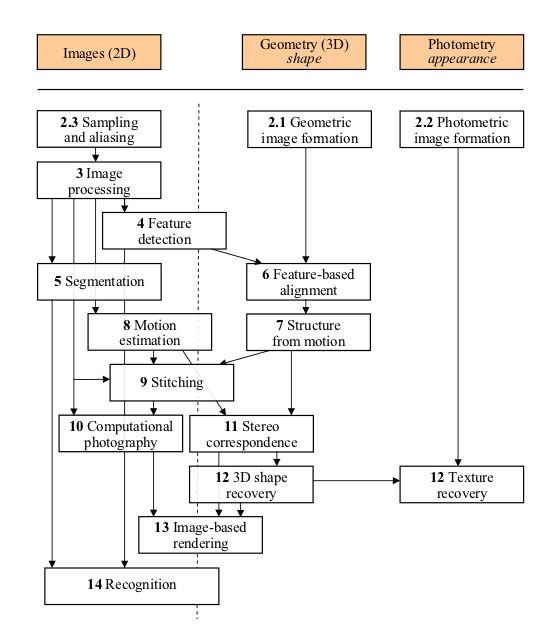
\includegraphics[scale=0.75]{figuras/diagrama_vc}}
    \caption{Divisão das áreas da Visão Computacional, relacionadas de acordo com suas dependências. Adaptado de \cite{SZELISKI}.}
    \label{img:diagrama_vc}
\end{figure}

Observando da esquerda para direita, podem ser vistos os três campos da Visão Computacional, divididos como: Imagens (\textit{Images}), Geometria (\textit{Geometry}) e Fotometria (\textit{Photometry}). A primeira área (\textit{Images}) cuida de problemas em um universo bidimensional. O tópico sobre Amostragem e Serrilhamento (\textit{Sampling and aliasing}) trata de questões referentes a fotografia digital. A parte de Processamento de Imagem (\textit{Image Processing}) foca na melhoria da qualidade da imagem para manipulações em sistemas de Visão Computacional. Já o processo de Detecção por Características (\textit{Feature Detection}), como o próprio nome sugere, dispõe de técnicas para reconhecimento de características em imagens.

Ainda, existe o processo de Segmentação (\textit{Segmentation}), que aborda técnicas de segmentação de imagens. Em outras palavras, esse processo é responsável por separar regiões relevantes de uma imagem. A Estimativa de Movimento (\textit{Motion Estimation}) é utilizada para alinhamento geométrico e calibração de câmeras e que em alguns momentos também pode ser encontrado em tarefas de um universo 3D (tridimensional). O processo de Junção de Imagens (\textit{Stitching}) cuida da criação de novas imagens a partir de uma ou mais imagens de entrada. Esse procedimento é bastante usado na área de mapas digitais e fotos de satélite, e tal como o processo de Estimativa de movimento, pode também ser utilizado em ambientes 3D.

Diretamente ligado ao processo de Junção de Imagens, encontra-se a Fotografia Computacional (\textit{Computational Photography}), que refere-se a captura, processamento e técnicas de manipulação da imagem computacional que melhoram ou aumentam a capacidade da fotografia digital. Como último processo de imagens 2D (bidimensional), temos o processo de Reconhecimento (\textit{Recognition}), tendo com tarefa principal analisar uma cena e reconhecer objetos.

Na próxima coluna, encontra-se os processos que tratam, em sua maioria, de casos em universo 3D. A Formação da Imagem Geométrica (\textit{Geometric image formation}) trata pontos, linhas e planos e como esses podem ser mapeados em imagens. A parte de Alinhamento Baseado em Características (\textit{Feature-based alignment}) trata das características recuperadas de imagens em processos anteriormente utilizados e busca identificá-las em outras diferentes imagens. Feito o processo de Alinhamento Baseado em Características, pode-se então utilizar o conjunto de técnicas no processo de Estrutura a Partir do Movimento (\textit{Structure from motion}), que cuida de encontrar estruturas tridimensionais de um objeto através de sinais de movimento continuamente.

Prosseguindo, está o processo Correspondência Estéreo (\textit{Stereo correspondence}), que pode ser entendido como a parte da Visão Computacional que analisa objetos em uma cena, sendo tratados por diversos pontos de vista. Na mesma linha de reconstrução de modelos 3D, está o componente de recuperação de formas 3D (\textit{3D shape recovery}). Diferente da Correspondência estéreo, esse componente funde diversas imagens de profundidade e de alcance. Por fim, está o componente da Renderização Baseada em Imagem (\textit{Image-based rendering}), diretamente ligado aos dois universos. O conjunto de técnicas nesse tópico cuida da geração de modelos 3D a partir de imagens 2D.

Além dessas áreas núcleo dos sistemas de Visão Computacional, existe a Fotometria, classe de técnicas de medição, que realiza a medição de objetos do mundo real usando apenas imagens. Em seus processos, estão a Formação da Imagem Fotométrica (\textit{Photometric image formation}) e a Recuperação de Texturas (\textit{Texture recovery}). O primeiro, descreve como os sensores geram valores de cor e intensidade, e como esses são formados em uma imagem. O segundo, está ligado a aparência dos objetos da superfície, após terem sido gerados como modelo 3D.

No Capítulo seguinte, são detalhados os principais processos de Visão Computacional. Por se tratar de disciplinas essenciais para o entendimento da área de Visão Computacional, foram escolhidos processos referentes ao universo bidimensional. A abordagem desses tópicos tem como finalidade servir de base conceitual para o desenvolvimento do estudo de caso, exposto no Capítulo 5.
 % VISÃO COMPUTACIONAL
	\chapter{PRINCIPAIS PROCESSOS DE VISÃO COMPUTACIONAL}

Este Capítulo contextualiza os principais processos da área de Visão Computacional. São descritas as técnicas mais utilizadas em cada um desses processos visando atingir o entendimento necessário para esse trabalho.

\section{Processamento de Imagem}

Processamento de Imagem é um processo da Visão Computacional que atua na maior parte dos projetos do universo bidimensional. Esse processo consiste em tratar a imagem buscando obter o máximo de qualidade possível sem se importar com a informação em si. Segundo \citeonline{JAIN}, o termo Processamento de Imagem refere-se ao processamento de uma imagem 2D através de um computador digital.

Embora essa área seja abordada como um processo de Visão Computacional, é normal encontrar algumas publicações que tratam esses dois processos como ciências isoladas. Uma dessas distinções é destacada por \citeonline{ALOIMONOS}, que atribuem como diferença básica o fato das tarefas envolvendo Processamento de Imagem serem de mais baixo nível que a Visão Computacional. Além disso, a Visão Computacional está relacionada com a percepção do ambiente, enquanto que o Processamento de Imagem é uma tarefa que possibilita essa percepção.

\citeonline{FREITAS} também relata que, apesar de ter em comum a imagem digital como fim ou como meio, ao processamento digital de imagem cabe a aquisição e a manipulação da informação adquirida na forma de \textit{pixels}\footnote{Menor ponto que forma uma imagem digital.}. Já Visão Computacional é uma área voltada à análise de imagens, interpretação de características e reconstituição do modelo de um objeto ou de uma cena.

Segundo \citeonline{OGE}, a etapa de aquisição de imagem tem como função converter uma imagem em uma representação numérica adequada para o processamento digital subsequente. Na etapa em que as imagens são tratadas, operações lógicas são realizadas em todos os \textit{pixels}, normalmente expressas sob forma algorítmica.

\subsection{Representação de Cores}

A forma como os seres humanos interpretam as cores varia de acordo com os seus sistemas visuais. Para representar essas cores em sistemas artificiais, criou-se os modelos de representações das cores. Segundo \citeonline{OGE}, o objetivo principal desses modelos é permitir a especificação de cores em um formato aceito por todos. Conceitualmente, os modelos de cores são representados através de sistemas tridimensionais de coordenadas, onde cada eixo refere-se a uma cor primária \cite{FOLEY}.

\subsubsection{Modelo RGB}

O modelo de cores RGB (\textit{red, green, blue}) é um sistema aditivo que possui a capacidade de representar a percepção humana com um alto grau de semelhança, além de conseguir iludir esta mesma percepção, fazendo com que as pessoas acreditem que possam enxergar várias cores em uma única reprodução \cite{FRED}. Por possuir essas características, este modelo foi adotado como padrão para reprodução de cores de diversos dispositivos eletrônicos, como câmeras digitais e monitores de vídeo.

Baseado em um sistema de coordenadas cartesianas, representado por um cubo, o modelo RGB possui como cores primárias o vermelho, o verde e o azul, que encontram-se localizadas uma em cada vértice do cubo \cite{OGE}. Nos demais vértices, encontram-se combinações de cores a partir das cores primárias. A tonalidade das cores variam também de acordo com sua intensidade, normalmente representadas através de um número no intervalo de 0 a 255. Intensidades mínimas, apresentam cores mais escuras enquanto que intensidades máximas apresentam cores mais claras.

A Figura \ref{img:modelo_rgb} apresenta essa forma de representação do modelo, utilizando o número 1 ao invés do 255 para representar a tonalidade máxima de uma cor. Além dos vértices representando as cores primárias, tem-se ainda mais dois vértices para representar as cores preta e branca, formados pela combinação das cores primárias em intensidades mínimas e máximas respectivamente. Além desses vértices, encontram-se também os vértices derivados da combinação de duas cores primárias. A cor magenta é resultado da combinação de vermelho com azul, enquanto que a cor amarela é combinação do vermelho com verde. Por fim tem-se o ciano, resultado da combinação da cor verde com azul.

\begin{figure}[H]
    \centering
    {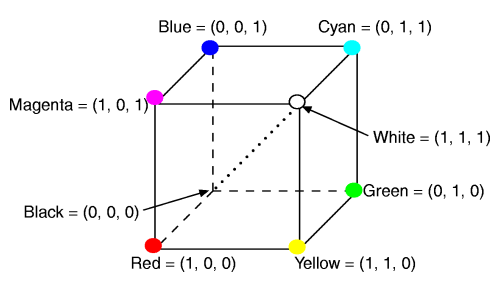
\includegraphics[scale=0.5]{figuras/modelo_rgb}}
    \caption{Representação do modelo RGB através do desenho de um cubo \cite{MOTTA}.}
    \label{img:modelo_rgb}
\end{figure}

\subsubsection{Modelo HSV}

O modelo HSV apresenta uma forma diferente de representar as cores, onde se tem a matiz (\textit{hue}), saturação (\textit{saturation}) e valor (\textit{value}). A matiz é responsável por determinar a tonalidade dominante de uma área, ou seja, a família em que aquela cor está inserida. Esse componente é medido através de valores entre 0 e 360. A saturação mede a pureza da cor da área. Já o valor define a luminância da cor. Nas modalidades de saturação e valor, a variação pode ocorrer entre 0\% e 100\%.

Conforme visto na Figura \ref{img:modelo_hsv}, o espaço de cor HSV é representado por um cone. O lado circular do cone apresenta as tonalidades, normalmente representadas por um ângulo, onde cada ângulo corresponde a uma cor no cone. A saturação é representada pela distância desde a borda ao centro do círculo, de modo que, quanto menor o valor de saturação, menor a presença de tons de cinza na imagem e mais próxima da cor branca. O brilho é determinado pela posição vertical em cores do cone. Na extremidade pontiaguda do cone, não há nenhum brilho, portanto a tonalidade das cores se aproximam da cor preta. No final do cone, na base, estão as cores mais brilhantes \cite{DARRIN}.

\begin{figure}[H]
    \centering
    {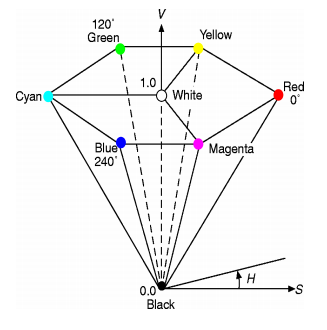
\includegraphics[scale=0.5]{figuras/modelo_hsv}}
    \caption{Representação do modelo HSV através do desenho de um cone \cite{MOTTA}.}
    \label{img:modelo_hsv}
\end{figure}

\subsection{Histograma}

Originalmente criados para melhor análise de dados estatísticos, os histogramas consistem em retângulos contíguos com base nas faixas de valores da variável e com área igual à frequência relativa da faixa. A altura de cada retângulo é denominada densidade de frequência definida pelo quociente da frequência relativa pela amplitude da faixa \cite{CECIRE}.

Em Processamento de Imagem a técnica de histograma é muito utilizada para indicar o percentual de diferentes tons de cinza dos \textit{pixels} em uma imagem através de um gráfico de barras, possibilitando dessa forma uma interpretação visual da distribuição dos valores dos tons de cores da imagem \cite{OGE}. Através da visualização do histograma de uma imagem é possível obter uma indicação de sua qualidade quanto ao nível de contraste e quanto ao seu brilho médio, determinados pela linha horizontal do gráfico. Entretanto, quando uma imagem é colorida, torna-se necessário a decomposição da mesma para que seja avaliado o histograma de cada um dos componentes da imagem separadamente (Figura \ref{img:ex_histograma}).

\begin{figure}[h]
    \centering
    {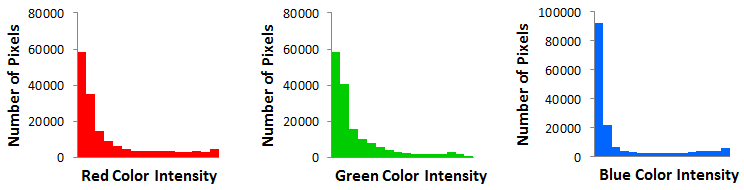
\includegraphics[scale=0.75]{figuras/ex_histograma}}
    \caption{Exemplo de gráficos de histogramas divididos nos canais de cores vermelho, verde e azul \cite{CLOUD}.}
    \label{img:ex_histograma}
\end{figure}

\section{Segmentação}

Além de ser um processo de Visão Computacional, a Segmentação possui uma ligação com a fase de Processamento de Imagem, visto que a qualidade da visualização interfere muito devido à dificuldade de se interpretar as características da imagem. O processo de Segmentação consiste em dividir a imagem em diferentes regiões, buscando separar áreas da imagem, que serão processados posteriormente no processo de Reconhecimento \cite{PUZICHA}.

Nesse processo, existe uma etapa denominada \textit{clustering}, fase de identificação da imagem, que pode ser de dois tipos: supervisionado ou não-supervisionado \cite{ZHOU}. Os processos supervisionados possuem conhecimento prévio sobre quais informações serão classificadas e agrupadas. Em contrapartida, os processos não-supervisionados não requerem nenhuma informação anterior sobre as informações que devem ser agrupadas.

A etapa de Segmentação pode ser realizada utilizando métodos baseados em histograma \cite{ROTHER}, onde são realizados cálculos utilizando um histograma a partir de todos os \textit{pixels} da imagem, e os picos e vales do histograma podem ser utilizados para definir um número d agrupamentos a ser encontrado. Além disso, esse processo também pode ser realizado através de lógica espacial \cite{KOLMOGOROV}, dividindo ou fundindo imagens a partir de pontos semelhantes.

Devido à dificuldade em fazer com que o computador reconheça os padrões e agrupe as imagens significativas, a Segmentação se torna um dos processos mais complexos da área de Visão Computacional. Tomando como base uma imagem que possui diversos objetos distintos, fazer com que o computador interprete e consiga separar esses objetos se tornou um desafio para os técnicos. Consequentemente, surgiram várias técnicas de agrupamentos que buscam no fim o mesmo resultado, ou seja, uma coleção de segmentos que quando combinados formam uma imagem inteira.

Existem várias técnicas e métodos para segmentar uma imagem tanto estática quanto dinâmica. A seguir serão apresentados alguns dos principais métodos de agrupamentos utilizados pelo processo de Segmentação.

\subsection{Segmentação por região}

A detecção por região pode ser feita extraindo uma região ou dividindo a imagem em várias regiões diferentes. As regiões normalmente apresentam como característica a continuidade do nível de cinza de seus pixels e podem ser detectadas pelos métodos de \textit{thresholding} ou dividindo e fundindo segmentos da imagem.

\subsubsection{\textit{Thresholding}}

Várias técnicas podem ser utilizadas para alcançar a seleção de segmentos que formam os objetos buscados pelo sistema. \textit{Thresholding}, também conhecido como limiarização, é o método de Segmentação de fácil compreensão, se comparado com as demais. O método consiste em utilizar imagens pós-processadas e convertidas para tonalidades de cinza em sequência, criando um limiar onde é separada da imagem principal uma imagem segmentada.

O \textit{thresholding} é um método baseado em histograma, onde o limiar de separação pode ser encontrado nos vales entre um pico e outro do histograma \cite{PADILHA}.

\subsubsection{Dividir e fundir}

Como mencionado no método de \textit{thresholding}, a maneira mais simples possível para segmentar uma imagem é selecionando um limiar e então calcular os componentes ligados. Entretanto, um único limiar raramente é o suficiente para a imagem por causa da iluminação e variações estatísticas do objeto \cite{SZELISKI}. O método de dividir e fundir agrupa em segmentos os \textit{pixels} que se encontram em regiões de características semelhantes, dividindo ou fundindo a imagem se preciso.

\subsection{Segmentação por contornos}

O contorno pode ser definido pela variação dos níveis de cinza entre duas regiões semelhantes. O método de detecção de contornos da imagem permite encontrar regiões com uniformidades de valores. Nesse método de Segmentação é localizado a região da imagem que possui variações nos valores. O objetivo do método é localizar as bordas ou curvas dos objetos nas imagens em forma de contornos finos e sem interrupções \cite{SZELISKI}.

Também é possível segmentar uma imagem por contornos através da detecção de pontos. Esse método é muito utilizado em objetos em movimento, avaliando a variação em suas direções principais \cite{ANTUNES}.

\subsection{Segmentação por textura}

A detecção por textura busca agrupar subconjuntos que possuam aproximadamente as mesmas características em qualquer lugar da imagem \cite{ANTUNES}. Essa técnica possui métodos como o estatístico, baseando-se na distribuição dos níveis de cinza da imagem para definir uma matriz que representa essa distribuição através da imagem, e então, a partir dessa matriz, identificar a probabilidade de um conjunto de \textit{pixels} compor uma determinada textura.

\section{Reconhecimento}

Realizar a análise e reconhecimento de objetos em uma cena tem sido uma das tarefas mais desafiadoras no domínio da Visão Computacional. Apesar de ser uma tarefa facilmente executada por crianças, conseguir que um computador realize a mesma tarefa não é igualmente simples \cite{SZELISKI}. A dificuldade no Reconhecimento se dá pela infinidade de classificações que os seres humanos empregam. Ainda é possível acontecer de objetos da mesma classe conterem atributos distintos, dificultando ainda mais a exatidão na fase de Reconhecimento e tornando improvável a análise através de uma base de dados de exemplos.

O objetivo da etapa de Reconhecimento é fazer com que o sistema classifique as informações adquiridas das etapas anteriores baseada em um conhecimento proposto ou com experiência em aprendizado.

Em muitos casos, o Reconhecimento depende do contexto onde o objeto está inserido e os elementos da cena. Se o objeto procurado for de conhecimento do computador, é possível procurar por pontos característicos e verificar se os mesmos se alinham de forma geométrica. Existem vários modelos utilizados para realizar um reconhecimento em uma imagem. Em seus estudos, \citeonline{WEBER} apresenta diversos modelos de Reconhecimento balanceados por funções probabilísticas.

Um dos modelos mais simples apresentados é caracterizado por um objeto constituído pela formação de várias peças que podem possuir características distintas, como aparência, forma e escala relativa. A partir da segmentação das peças do objeto é iniciada a fase de detecção, que em uma primeira etapa utiliza detectores especializados para cada uma das peças formadas. Após as peças serem reconhecidas e suas informações armazenadas, a segunda etapa é iniciada para a detecção do objeto formado através da união das informações de cada peça recolhida. Outra etapa importante no processo é a localização do objeto na imagem, que é realizada usando as peças detectadas que correspondem ao objeto em primeiro plano na imagem.

Através desse modelo, conseguiu-se um reconhecimento razoavelmente rápido e simples. Além disso, a partir desse modelo, Weber propôs outros modelos que utilizavam cálculos com funções buscando um custo de processamento menor.
 % PRINCIPAIS PROCESSOS DE VISÃO COMPUTACIONAL
	\chapter{BIBLIOTECAS DE VISÃO COMPUTACIONAL}

No mercado de software atual, existem bibliotecas que auxiliam o desenvolvimento de sistemas de Visão Computacional, direcionadas em diversos focos. Muitas dessas ferramentas têm como objetivo suportar questões específicas do campo de estudo de Visão Computacional.

Apesar de não ser o foco deste trabalho, algumas dessas bibliotecas merecem destaque. Uma delas se trata do VLFeat\footnote{\url{http://github.com/mmmikael/vlfeat}}, biblioteca que possui em sua implementação algoritmos populares de Visão Computacional. Outra biblioteca a ser destacada é o VIGRA\footnote{\url{http://hci.iwr.uni-heidelberg.de/vigra}}, que enfatiza o uso de algoritmos flexivéis, construídos usando programação genérica \cite{MUSSER}.

Outras bibliotecas por sua vez possuem recursos que ampliam seu uso em diversas áreas no desenvolvimeto de sistemas de Visão Computacional. Essas bibliotecas são suportadas por diversas linguagens, tanto de baixo nível como de alto nível. Visando a boa produtividade e simples manuseio, optou-se pela abordagem de linguagens de programação de alto nível. Por se tratar de uma linguagem de simples utilização e aprendizado, foi escolhida a linguagem de programação Python neste trabalho. Essa linguagem conta com diversos recursos de uso simples e possui boa integração com as bibliotecas mais utilizadas na área de Visão Computacional.

No grupo de bibliotecas suportadas pela linguagem Python, a que mais se destaca é o OpenCV. Através do uso de interfaces, a utilização da ferramenta tem facilitado o desenvolvimento de aplicações de Visão Computacional, além de permitir o melhor entendimento da área. Existe também o \textit{framework} SimpleCV, com a missão de simplificar ainda mais o uso das interfaces do OpenCV para Python.

Neste Capítulo, são mostradas a utilização e instalação dessas ferramentas de uso geral para o desenvolvimento de sistemas de Visão Computacional suportadas pela linguagem Python.

\section{OpenCV}

Considerada como uma das mais completas bibliotecas na área de Visão Computacional \cite{THORNE} \cite{SEYDOUX}, o OpenCV\footnote{\url{http://opencv.willowgarage.com}} se destaca pelo seu uso abrangente, possuindo mais de 500 funções que implementam técnicas em diversas áreas de Visão Computacional. Dentre as áreas que a biblioteca atua estão: Processamento de Imagem, Segmentação, Transformação, Rastreamento, Calibração de Câmera, entre outras.

Desenvolvida pela Intel, a biblioteca do OpenCV foi criada para prover uma infraestrutura para criação rápida de aplicações de Visão Computacional. Por possuir o foco em aplicações em tempo real, seu código é escrito na linguagem C e C++. Essas linguagens são mais próximas das linguagens de máquina, desta forma, tendem a ter um desempenho superior às linguagens mais atuais, que necessitam ser interpretadas por uma máquina virtual. A utilização do OpenCV pode ainda ser flexibilizada através de interfaces, criadas para se comunicar com outras linguagens de programação como Java, Python e Ruby.

O uso do OpenCV pode ser otimizado com a utilização da biblioteca proprietária \textit{multi-core ready} IPP (\textit{Integrated Performance Primitives}), que possui funções altamente otimizadas para multimídia, processamento de dados e aplicações de comunicação \cite{IPP}. Em estudos realizados por \citeonline{BRADSKI}, a biblioteca é comparada trabalhando de forma independente e integrada com a biblioteca IPP. Essa comparação é apresentada na Figura \ref{img:comparativo}, onde é possível observar o ganho razoável de performance da biblioteca ao ser utilizada em conjunto com a IPP.

\begin{figure}[H]
    \centering
    {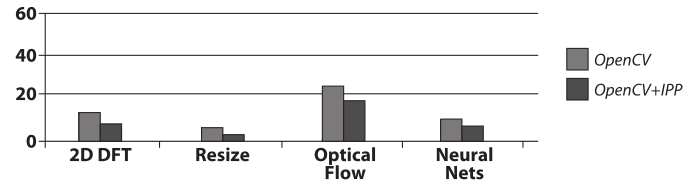
\includegraphics[scale=0.5]{figuras/comparativo}}
    \caption{Comparativo de desempenho entre a ferramenta OpenCV com e sem a biblioteca proprietária da Intel. Adaptado de \cite{BRADSKI}.}
    \label{img:comparativo}
\end{figure}

\subsection{Estrutura}

Baseando-se em relatos de \citeonline{BRADSKI}, o OpenCV é estruturado em cinco componentes principais. As partes de mais alto nível são dividias em: \textit{CV}, \textit{MLL} e \textit{HighGUI}. Como é possível ver na Figura \ref{img:estrutura_opencv}, no componente \textit{CV} está toda a parte de Processamento de Imagem e algoritmos de Visão Computacional. O componente \textit{MLL} contém ferramentas de \textit{clustering} e métodos de classificadores estatísticos. A parte de \textit{HighGUI}, como o nome sugere, contém componentes de interface com usuário, assim como rotinas de entrada e saída de vídeos e imagens. Da mesma forma, no \textit{CXCORE} estão contidas todas as estruturas de dados usadas no OpenCV. Nesse componente também existem algoritmos para manipulação de arquivos XML, sendo possível realizar leitura e gravação de dados. Outro recurso reunido nesse componente bastante utilizado pelos desenvolvedores são as funções de desenho. Através delas, é possível, por exemplo, destacar em uma imagem ou vídeo uma região de interesse (ROI).

Além dos componentes descritos, o OpenCV ainda conta com um componente auxiliar, nomeado de \textit{CvAux}, contendo métodos experimentais. A ideia desse módulo é conter funções de Visão Computacional em fases de testes que podem ser usadas pelos desenvolvedores, e com a aceitação ou não de cada função, a mesma é inserida nos módulos principais como uma função oficial do OpenCV.

\begin{figure}[h]
    \centering
    {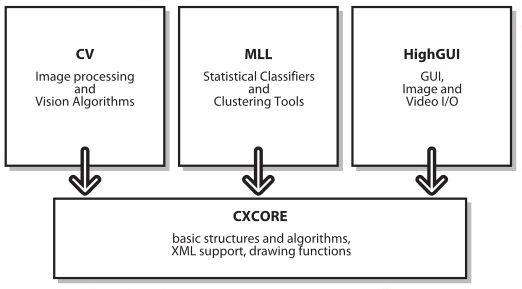
\includegraphics[scale=0.75]{figuras/estrutura_opencv}}
    \caption{Estrutura da biblioteca OpenCV \cite{BRADSKI}.}
    \label{img:estrutura_opencv}
\end{figure}

Como interfaces do OpenCV para linguagem Python, existem duas que cumprem esse papel. A primeira, declarada como \textit{cv2.cv}, é uma implementação mais antiga e trabalha com classes da própria interface. A segunda, nomeada como \textit{cv2}, possui mais dinamicidade em seu uso, permitindo atribuições a tipos de dados nativos do Python. Exemplificando a comparação das duas interfaces, ao carregar uma imagem em ambas, observa-se a diferença em como cada uma delas trata os dados (Código \ref{code:cv_e_cv2}).

\begin{code}{python}{O tipo das variáveis se diferem devido o uso de \textit{bindings} diferentes.}{code:cv_e_cv2}
In [1]: img = cv.LoadImage('logo_iff.png')
In [2]: img
Out[2]: <iplimage(nChannels=3 width=291 height=385 widthStep=876 )>

In [3]: img2 = cv2.imread('logo_iff.png')
In [4]: img2
Out[4]: array([[[255, 255, 255],...,[255, 255, 255]]], dtype=uint8)

In [5]: type(img2)
Out[5]: <type 'numpy.ndarray'>
\end{code}

\subsection{Instalação}
\label{section:install_opencv}

Nas pesquisas realizadas, foi utilizado o sistema operacional Ubuntu em sua versão 11.10, em conjunto da biblioteca OpenCV em sua versão 2.4.2 e a linguagem de programação Python em sua versão 3.0. Buscando uma instalação mais completa e com a maioria dos recursos disponíveis, procurou-se reunir a maior parte das dependências da ferramenta. Contudo, não foi possível realizar a instalação da biblioteca IPP, por se tratar de uma biblioteca proprietária.

Antes de iniciar a instalação do OpenCV, recomenda-se a remoção das bibliotecas usadas pela ferramenta que já estejam instaladas no sistema operacional \cite{ERALP}. O Código \ref{code:remover_pacotes_padrao} apresenta a remoção das bibliotecas comumente encontradas no sistema operacional Linux Ubuntu 11.10.

\begin{terminal}{Remoção de pacotes instalados por padrão no sistema operacional Linux Ubuntu 11.10.}{code:remover_pacotes_padrao}
sudo apt-get remove ffmpeg x264 libx264-dev
\end{terminal}

Para a instalação da biblioteca, é necessário baixar o pacote compactado em sua página oficial. A versão usada no trabalho foi a 2.4.2. A instalação da biblioteca é realizada através de uma ferramenta de construção de sistemas, o CMake (Código \ref{code:install_cmake}). Além disso, existem outras dependências que precisam ser instaladas antes da execução da instalação do OpenCV (Código \ref{code:install_dependencias}).

\begin{terminal}{Instalação da ferramenta CMake.}{code:install_cmake}
sudo apt-get install cmake
\end{terminal}

\begin{terminal}{Instalação de dependências do OpenCV.}{code:install_dependencias}
sudo apt-get install build-essential
sudo apt-get install python-dev python-numpy python-sphinx
sudo apt-get install libgtk2.0-0 libgtk2.0-dev
sudo apt-get install libjpeg8 libjpeg8-dev
sudo apt-get install libgstreamer0.10-0 libgstreamer0.10-dev gstreamer0.10-tools \
  gstreamer0.10-plugins-base libgstreamer-plugins-base0.10-dev \
  gstreamer0.10-plugins-good gstreamer0.10-plugins-ugly gstreamer0.10-plugins-bad \
  gstreamer0.10-ffmpeg
sudo apt-get install libjasper-dev
sudo apt-get install libavcodec-dev
sudo apt-get install libdc1394-22-dev
sudo apt-get install libavformat-dev
sudo apt-get install libv4l-dev
sudo apt-get install libswscale-dev
\end{terminal}

O FFmpeg, conjunto de ferramentas para gravação, conversão e criação de stream de áudio e vídeo, uma das dependências do OpenCV, necessita da instalação prévia de outras bibliotecas para seu funcionamento. Essas dependências são descritas no Código \ref{code:dependencias_ffmpeg}. Após a instalação destas dependências, instala-se o FFmpeg (Código \ref{code:install_ffmpeg}).

\begin{terminal}{Instalação das dependências do FFmpeg.}{code:dependencias_ffmpeg}
sudo apt-get install libfaac-dev libjack-jackd2-dev libmp3lame-dev \
  libopencore-amrnb-dev libopencore-amrwb-dev libsdl1.2-dev libtheora-dev \
  libva-dev libvdpau-dev libvorbis-dev libx11-dev libxfixes-dev libxvidcore-dev \
  texi2html yasm zlib1g-dev libx264-dev
mkdir ~/src
cd ~/src
wget ftp://ftp.videolan.org/pub/videolan/x264/snapshots/ \
	x264-snapshot-20120820-2245-stable.tar.bz2
tar xvf x264-snapshot-20120820-2245-stable.tar.bz2
cd x264-snapshot-20120820-2245-stable/
./configure --enable-static
make
sudo make install
\end{terminal}

\begin{terminal}{Instalação do FFmpeg.}{code:install_ffmpeg}
cd ~/src
wget http://ffmpeg.org/releases/ffmpeg-0.11.tar.bz2
tar xvf ffmpeg-0.11.tar.bz2
cd ffmpeg-0.11
./configure --enable-gpl --enable-libfaac --enable-libmp3lame \
  --enable-libopencore-amrnb --enable-libopencore-amrwb --enable-libtheora \
  --enable-libvorbis --enable-libx264 --enable-libxvid --enable-nonfree \
  --enable-postproc --enable-version3 --enable-x11grab
make
sudo make install
\end{terminal}

Outra dependência do OpenCV é a biblioteca V4L, uma interface de captura de vídeo para programação de aplicativos para Linux. Pode ser baixada e instalada através dos comandos mostrados no Código \ref{code:install_v4l}.

\begin{terminal}{Instalação do V4L.}{code:install_v4l}
cd ~/src
wget http://www.linuxtv.org/downloads/v4l-utils/v4l-utils-0.8.8.tar.bz2
tar xvf v4l-utils-0.8.8.tar.bz2
cd v4l-utils-0.8.8
make
sudo make install
\end{terminal}

Agora é possível executar a instalação do OpenCV. Após realizada a descompactação do pacote, na pasta do OpenCV, crie um diretório onde estarão contidos os arquivos (Código \ref{code:install_opencv1}).

\begin{terminal}{Comandos iniciais para instalação do OpenCV.}{code:install_opencv1}
mkdir release
cd release
\end{terminal}

O comando \textit{cmake} irá construir os executáveis da instalação do OpenCV (Código \ref{code:install_opencv2}).

\begin{terminal}{Execução da instalação do OpenCV através do CMake.}{code:install_opencv2}
cmake -D CMAKE_BUILD_TYPE=RELEASE -D CMAKE_INSTALL_PREFIX=/usr/local \
  -D BUILD_NEW_PYTHON_SUPPORT=ON -D BUILD_EXAMPLES=ON ..
\end{terminal}

Ao executar o comando acima, é possível visualizar quais depedências foram reconhecidas. No geral, as mais importantes são: GTK+ 2.x, FFMPEG, GStreamer e V4L/V4L2. Por fim, é necessário executar os comandos que irão de fato instalar a biblioteca na máquina (Código \ref{code:install_opencv3}).

\begin{terminal}{Comandos finais para instalação do OpenCV.}{code:install_opencv3}
make
sudo make install
\end{terminal}

\subsection{Uso prático}

O OpenCV conta com diversos exemplos em várias linguagens em seu subdiretório (\textit{OpenCV-2.4.2/samples}). Sua documentação também é bastante rica, e pode ser acessada através de seu site\footnote{\url{http://opencv.itseez.com}}, contendo descrição e exemplos dos recursos da biblioteca.

Tomando como base esse material, foi selecionado um conjunto expressivo de comandos da biblioteca, para que seja possível uma rápida familiarização com a ferramenta. Começando com um exemplo básico, é possível carregar e mostrar uma imagem na tela através dos comandos do Código \ref{code:opencv_imread}.

\begin{code}{python}{Carregamento básico de imagem utilizando OpenCV.}{code:opencv_imread}
import cv2
img = cv2.imread('caminho_da_imagem')
cv2.imshow('titulo', img)
cv2.waitKey(0)
\end{code}

A primeira linha importa a interface do OpenCV, que no caso é a \textit{cv2}. Caso seja necessário o uso da interface alternativa, basta substituir \textit{cv2} por \textit{cv2.cv}. O Código \ref{code:opencv_print_img} mostra o conteúdo do \textit{array} da imagem carregada, com os valores RGB de cada \textit{pixel}.

\begin{code}{python}{Comando para visualização dos valores atribuidos a variável \textit{img}.}{code:opencv_print_img}
print img
\end{code}

A saída será um \textit{array} (Código \ref{code:saida_array}), onde para cada grupo de valores RGB é montado um \textit{array}, que por sua vez é agrupado e compõe uma linha vertical da imagem. Então cada \textit{array} é agrupado e assim se forma um \textit{array} que representa por completo a imagem carregada. Dessa forma, se torna flexível a realização de diferentes tipos de operações, como recortar e converter tipos (Código \ref{code:array_oper}).

\begin{code}{python}{Saída do \textit{array}, representando uma imagem carregada pela interface cv2.}{code:saida_array}
[[[255 255 255]
  [255 255 255]
  [255 255 255]
  ...,
  [255 255 255]
  [255 255 255]
  [255 255 255]]
 ...,
 [[255 255 255]
  [255 255 255]
  [255 255 255]
  ...,
  [255 255 255]
  [255 255 255]
  [255 255 255]]]
\end{code}

\begin{code}{python}{Recorte na imagem pode ser realizado através de manipulações com \textit{arrays}.}{code:array_oper}
parte_um = img[:len(img)/2]
parte_dois = img[len(img)/2:]
\end{code}

Pelo fato da variável \textit{img} ser de um tipo conhecido pela linguagem Python, as manipulações com seus valores se tornam simples. Para salvar as variáveis, cada uma contendo metade da imagem, utiliza-se o que é exposto no Código \ref{code:save_imgs}.

\begin{code}{python}{Imagens são salvas utilizando o método do OpenCV que realiza essa operação.}{code:save_imgs}
cv2.imwrite('DIR_PROJETO/images/img1.jpg', parte_um)
cv2.imwrite('DIR_PROJETO/images/img2.jpg', parte_dois)
\end{code}

Quanto as conversões de espaço de cor, a biblioteca possui funções e variáveis próprias para essa tarefa. Por padrão, a imagem carregada é armazenada na ordem BGR, que é contrária a mais conhecida, RGB. Através do comando \textit{cvtColor()} é possível obter, por exemplo, essa ordem de cores (Código \ref{code:convert_bgr2rgb}).

\begin{code}{python}{Operação para inversão da ordem do espaço de cor BGR para RGB.}{code:convert_bgr2rgb}
img_gray = cv2.cvtColor(img, cv2.COLOR_BGR2RGB)
\end{code}

Em algumas documentações da biblioteca, é comum encontrar os nomes das variáveis usadas para transformação do espaço de cor precedidos por CV, principalmente as que se referem a linguagem C. Contudo, na interface para Python, os nomes das varíaveis referentes a esse tipo de operação se encontram com o prefixo COLOR. Uma lista completa de todas as variáveis usadas em conjunto com o método \textit{cvtColor()} pode ser encontrada na documentação oficial da biblioteca, ou então no próprio ambiente de configuração, caso o mesmo tenha a capacidade de autocompletar o código a ser escrito.

Outras operações bastante usadas com a ferramenta, são relacionadas a análises estruturais e descritores de formas. Através de contornos, que segundo \citeonline{BRADSKI} tratam-se de uma lista de pontos que representam, de uma forma ou outra, uma curva em uma imagem, o OpenCV consegue recuperar informações de objetos em uma imagem. Em outras palavras, o seu limite. Essa técnica se torna muito poderosa em ocasiões em que é preciso detectar e reconhecer objetos em imagens e vídeo. O Código \ref{code:contours} mostra um exemplo de como obter os contornos de uma imagem.

\begin{code}{python}{Recuperação de contornos dos objetos contidos na imagem com o logotipo do IFF.}{code:contours}
img = cv2.imread('DIR_PROJETO/images/logo_iff.png')
img_gray = cv2.cvtColor(img, cv2.COLOR_BGR2GRAY)
ret, thresh = cv2.threshold(img_gray, 127, 255, cv2.THRESH_BINARY)
contours, hierarchy = cv2.findContours(thresh, cv2.RETR_TREE, cv2.CHAIN_APPROX_NONE)
\end{code}

A primeira linha, como visto anteriormente, carrega uma imagem, que no exemplo, será o logotipo do Instituto Federal Fluminense (Figura \ref{img:logo_iff}). Então a imagem é convertida para escala de cinza, para que possa ser usada no próximo método, \textit{threshold()}. Esse método delimita uma parte da imagem de acordo com os parâmetros passados. No exemplo, é especificado pelos parâmetros manter os \textit{pixels} que estiverem entre 127 e 255, colocando-os em preto. Os que não forem deste grupo, são retirados. Esse método transforma uma imagem em escala de cinza em uma imagem binária\footnote{Imagem digital com todos os valores de \textit{pixel} 0 ou 1.}, mantendo apenas os \textit{pixels} que sejam de interesse. Com esses parâmetros, obtem-se uma imagem com apenas parte do logotipo (Figura \ref{img:logo_parcial_bin}). Para que seja possível recuperar todos os seus elementos, faz-se necessário alterar os parâmetros passados. Tendo a parte vermelha 234, 31, 42 como valores RGB, seu valor em escala de cinza é 93, baseando-se na fórmula de conversão de RGB para escala de cinza \cite{KUMAR}. Já os quadrados verde, possuem valor 155 em escala de cinza e 115, 196 e 48 como valores RGB. Portanto, para recuperar todo o logotipo, altera-se os parâmetros para 155 e 255. Os resultados são vistos na Figura \ref{img:logo_bin}.

\begin{figure}[ht]
    \centering
    {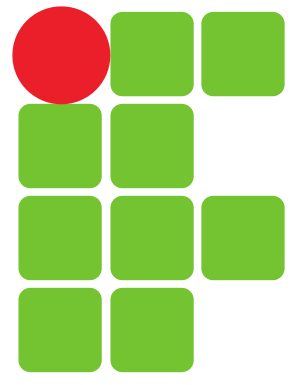
\includegraphics[scale=0.25]{figuras/logo_iff}}
    \caption{Logotipo do Instituto Federal Fluminense.}
    \label{img:logo_iff}
\end{figure}

\begin{figure}[H]
	\centering
	\subfigure[Logotipo parcialmente binarizado.]{
		
\includegraphics[scale=0.25]{figuras/logo_parcial_bin}
		\label{img:logo_parcial_bin}
	}\hspace{3em}
	\subfigure[Logotipo totalmente binarizado.]{
		
\includegraphics[scale=0.25]{figuras/logo_bin}
		\label{img:logo_bin}
	}
	\caption{Limiarização com diferentes \textit{thresholds} no logotipo do IFF.}
	\label{img:threshold_logotipo}
\end{figure}

Realizada a etapa de \textit{threshold}, pode-se então recuperar os contornos dos elementos em preto na imagem. Aplicando o método \textit{findContours()}, descrito na linha 4 do Código \ref{code:contours}, é retornada uma lista com os limites de todos os elementos. Através do Código \ref{code:num_elem}, é possível ver o comando utilizado para saber a quantidade de elementos que o OpenCV recuperou.

\begin{code}{python}{Comando para imprimir saída, contendo o número de elementos da figura.}{code:num_elem}
print len(contours)
\end{code}

Como o exemplo utiliza uma imagem binarizada com todos os objetos da imagem, o resultado é dez, representando a quantidade de elementos do \textit{array}. Apesar de haver dez elementos em preto identificáveis, a ferramenta uniu dois deles, e obteve o contorno do fundo branco, como é possível ver na Figura \ref{img:track_um_threshold}, após os contornos serem desenhados. Entretanto, pelo fato dos elementos unidos serem de cores diferentes, é possível separá-los, aplicando dois \textit{thresholds} em momentos diferentes do código. Realizada a etapa de recuperação dos contornos, os mesmos são desenhados na imagem. O resultado final é exposto na Figura \ref{img:track_dois_threshold}, enquanto o Código \ref{code:completo} contém todas as operações necessárias para se chegar a este resultado.

\begin{figure}[H]
	\centering
	\subfigure[Contornos obtidos com um \textit{threshold}.]{
		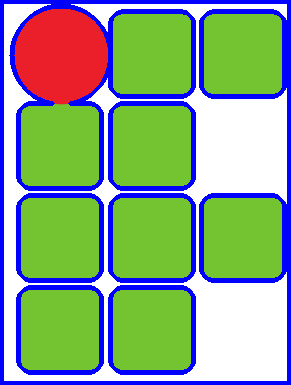
\includegraphics[scale=0.25]{figuras/track_um_threshold}
		\label{img:track_um_threshold}
	}\hspace{3em}
	\subfigure[Contornos obtidos com dois \textit{thresholds}.]{
		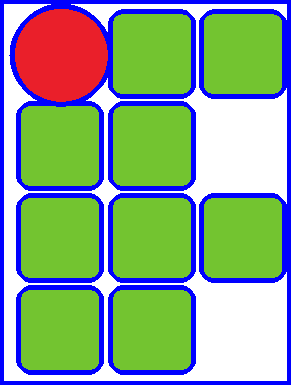
\includegraphics[scale=0.25]{figuras/track_dois_threshold}
		\label{img:track_dois_threshold}
	}
	\caption{Contornos desenhados em seus respectivos elementos. Nos contornos da Figura \ref{img:track_um_threshold}, os dados foram obtidos com apenas um \textit{threshold}, já na Figura \ref{img:track_dois_threshold} foram usados dois \textit{thresholds}.}
	\label{img:threshold_logotipo}
\end{figure}

\begin{code}{python}{Toda a lógica para obtenção dos contornos e desenho dos mesmos.}{code:completo}
img = cv2.imread('DIR_PROJETO/images/logo_iff.png')
img_gray = cv2.cvtColor(img, cv2.COLOR_BGR2GRAY)
ret, thresh_ball = cv2.threshold(img_gray, 93, 255, cv2.THRESH_BINARY)
contours, hierarchy = cv2.findContours(thresh_ball, cv2.RETR_TREE, cv2.CHAIN_APPROX_NONE)
cv2.drawContours(img, contours[1], -1, (255,0,0),3)
ret, thresh_squares = cv2.threshold(img_gray, 155, 255, cv2.THRESH_BINARY)
contours2, hierarchy = cv2.findContours(thresh_squares, cv2.RETR_TREE, \
	cv2.CHAIN_APPROX_NONE)
cv2.drawContours(img, contours2, -1, (255,0,0),3)
cv2.imwrite('DIR_PROJETO/images/saida.png', img)
\end{code}

Ainda, através dos contornos, é possível recuperar os momentos da imagem. A biblioteca realiza essa tarefa através da função \textit{moments()}. O Código \ref{code:moments} recupera os momentos do segundo contorno da lista, que contém o círculo vermelho do logotipo. Esse método retorna um dicionário, que é um tipo de dados da linguagem Python. Ao exibir as informações contidas nessa lista, é possível visualizar todos os pares de chave e valor do dicionário (Código \ref{code:saida_moments}).

\begin{code}{python}{Os momentos são recuperados ao passar um contorno que representa um objeto da imagem.}{code:moments}
moments = cv2.moments(contours[1])
\end{code}

\begin{code}{python}{Os valores dos momentos do segundo elemento do logotipo do IFF são mantidos por um dicionário, um tipo de dados do Python.}{code:saida_moments}
{'mu02': 4466250.579995997, 'mu03': 2.099651949538806e-06, 'm11': 24999544.25,
 'nu02': 0.07959091389346826, 'm12': 1642430867.25, 'mu21': -6560.77209803462,
 'mu20': 4465517.828794554, 'nu20': 0.07957785588502587, 'm30': 2505168506.5,
 'nu21': -1.350844812113205e-06, 'mu11': -4485.94523428008,
 'mu12': -19483.180956840515, 'nu11': -7.994188290096345e-05,
 'nu12': -4.011533021684291e-06, 'm02': 26989947.0, 'm03': 1969781748.75,
 'm00': 7491.0, 'm01': 410761.5, 'mu30': 23255.18666744232,
 'nu30': 4.788178555058973e-06, 'm10': 455995.0, 'm20': 32223018.833333332,
 'm21': 1766364339.4166667}
\end{code}

Essas chaves são de três tipos: \textit{mu} (momentos centrais), \textit{nu} (momentos centrais normalizados) e \textit{m} (momentos espaciais). Ainda existem os momentos invariantes, também conhecidos como momentos \textit{Hu}, que podem ser recuperados através do método \textit{HuMoments()}. Mais sobre momentos no OpenCV podem ser encontrados no trabalho realizado por \citeonline{KILIAN}.

Através desses momentos, é possível obter características dos objetos, como sua área e centróide. A área do objeto é contida na chave \textit{m00}. Tendo esse valor, encontra-se então as coordenadas x e y do centro de massa do objeto (Código \ref{code:param_moments}).

\begin{code}{python}{Operações com os momentos do segundo elemento da lista de contornos.}{code:param_moments}
area = moments['m00']
x = moments['m10'] / area
y = moments['m01'] / area
\end{code}

Caso esteja definido a forma do objeto a ser encontrado, como um círculo, se torna interessante a recuperação de outros dados específicos dessa forma. Com isso, o resultado final tende a ser mais preciso, devido ao aumento de informações recuperadas do objeto a ser detectado. Como no exemplo apresentado é utilizado um objeto em forma circular, uma das informações relevantes a ser recuperada a respeito desse objeto é o seu raio. Isso é feito usando a fórmula da geometria, junto ao valor da área do contorno. Então, desenhando os valores encontrados, determina-se exatamente o centro e contorno do círculo vermelho em relação a figura em que ele está inserido (Código \ref{code:draw_circle}). O resultado é exposto na Figura \ref{img:track_final}.

\begin{code}{python}{Desenho feito na imagem de exemplo usando os parâmetros calculados a partir do momentos do contorno.}{code:draw_circle}
raio = sqrt(area/3.14)
cv2.circle(img, (int(x),int(y)), int(raio), (255,0,0), 3)
cv2.circle(img, (int(x),int(y)), 3, (255,0,0), -1)
\end{code}

\begin{figure}[H]
    \centering
    {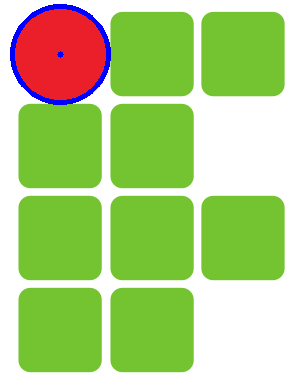
\includegraphics[scale=0.25]{figuras/track_final}}
    \caption{Rastreamento feito no círculo vermelho do logotipo do IFF.}
    \label{img:track_final}
\end{figure}

A biblioteca ainda conta com recursos para manipulações com vídeo, onde pode-se utilizar arquivos de vídeo ou câmeras, como a de um notebook. Para o caso de uma câmera de um nootebook usa-se o comando mostrado no Código \ref{code:video_opencv}.\newline\newline

\begin{code}{python}{Inicialização do vídeo através da biblioteca OpenCV.}{code:video_opencv}
video = cv2.VideoCapture(0)
\end{code}

Um número inteiro é passado pela função que recupera o vídeo, representando o identificador do dispositivo de vídeo. A partir desse objeto, cria-se então uma rotina para captura e apresentação dos \textit{frames} do vídeo em uma nova janela (Código \ref{code:loop_video}).

\begin{code}{python}{Lógica para processamento e visualização dos \textit{frames} do vídeo.}{code:loop_video}
while video.grab():
	flag, frame = video.retrieve()
	if flag:
		cv2.imshow('Video', frame)
		cv2.waitKey(1)
\end{code}

Tendo em mente que um vídeo é composto por diversas imagens em sequência, os mesmos tratamentos feitos em imagens também podem ser utilizados em vídeos, como aplicação de filtros e desenhos. Isso abrange as possibilidades em inúmeras atividades, que podem evoluir até sistemas completos de Visão Computacional.

\section{SimpleCV}

SimpleCV\footnote{\url{http://simplecv.org}} é um \textit{framework}\footnote{Coleção abstrata de classes, interfaces e padrões dedicados a resolver um conjunto de problemas através de uma arquitetura flexível e extensível.} de código aberto que foi desenvolvido pelos engenheiros da Sight Machine, e está sob a licença BSD (\textit{Berkeley Software Distribution}). O \textit{framework} é portável nas plataformas Mac, Windows e distribuições Linux Ubuntu e Arch Linux.

O objetivo do \textit{framework} é tornar mais fácil aos programadores o desenvolvimento de sistemas de Visão Computacional, simplificando muitas das tarefas mais comuns. \citeonline{DEMAAGD} destacam que, por ser uma biblioteca simples, não é necessário possuir muitos conhecimentos em Python e especialização na área da computação, sendo preciso apenas o interesse em Visão Computacional.

\subsection{Estrutura}

Em sua implementação, o SimpleCV utiliza bibliotecas existentes para Python na área de Visão Computacional, reunindo os recursos mais importantes de cada uma delas. A Figura \ref{img:estrutura_simplecv} expõe a relação do SimpleCV com as bibliotecas existentes no mercado. É destacado pelo diagrama a nova camada criada pelo SimpleCV, que acessa os recursos necessários das bibliotecas para Python. Dessa forma, grande parte das tarefas de Visão Computacional comumente realizadas, tornam-se mais simples.

\begin{figure}[h]
    \centering
	{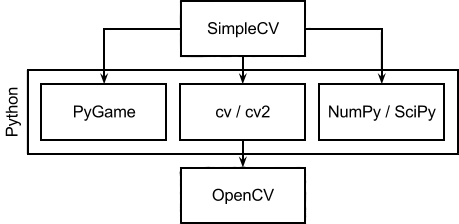
\includegraphics[scale=0.75]{figuras/estrutura_simplecv}}
    \caption{Bibliotecas usadas pelo SimpleCV divididas em camadas.}
    \label{img:estrutura_simplecv}
\end{figure}

Segundo sua documentação oficial\footnote{\url{http://simplecv.org/docs}}, o SimpleCV se encontra em sua versão 1.3 dividido em conjuntos de classes. Essa classes são separadas da seguinte forma: \textit{Features}, \textit{MachineLearning}, \textit{Segmentation} e \textit{Shell}. O pacote \textit{Features}, conta com métodos para classificação de objetos em imagens, baseando-se em suas características. O conjunto de classes contidos no pacote \textit{MachineLearning} implementam alguns algoritmos de classificação, como o \textit{k-nearest neighbor} e \textit{Naive Bayes}. O pacote \textit{Segmentation} contém classes para segmentação de imagens, podendo ser diferenciada por cor ou comparando diferenças entre dois \textit{frames}. A classe \textit{Shell} permite que a biblioteca seja usada via terminal, tendo dessa forma, resposta rápida para dúvidas que surgirem durante o desenvolvimento, realização de testes rápidos e acesso a última documentação dos objetos do SimpleCV. Essa implementação é baseada no IPython.

Além desses pacotes, existem ainda as classes básicas da ferramenta, sendo elas: \textit{Camera}, \textit{Color}, \textit{ColorModel}, \textit{Display}, \textit{DrawingLayer}, \textit{EXIF}, \textit{Font}, \textit{ImageClass} e \textit{Stream}. Cada uma delas possui uma finalidade distinta. Com a classe \textit{Camera}, por exemplo, é possível trabalhar com vídeo de diversos dispositivos, como a de um notebook, de câmeras que enviam sinais pela Internet (\textit{stream}) ou até mesmo da câmera do Kinect\footnote{Sensor de movimentos de última geração, desenvolvimento inicialmente para jogos eletrônicos.}, dispositivo desenvolvido pela Microsoft. Outras classes fornecem manipulações com interface, mostrando resultados de imagens e vídeo em janelas do sistema operacional e eventos com o mouse, e desenhos básicos de formas e texto.

\subsection{Instalação}

Existem diversas formas de realizar a instalação do SimpleCV no Linux Ubuntu 11.10. Independente do método escolhido para a instalação do \textit{framework}, existem dependências que precisam ser instaladas previamente. São elas: Python (2.7 ou superior), Python Setup Tools, PyGame, NumPy, SciPy, Easy Install e o OpenCV. Essas dependências podem ser instaladas através do comando mostrado no Código \ref{code:depend_simplecv}.

\begin{terminal}{Instalação das dependências do SimpleCV.}{code:depend_simplecv}
sudo apt-get install python-setuptools python-pygame python-scipy
\end{terminal}

Por padrão as dependências restantes já vem instaladas na versão 11.10 do Linux Ubuntu, sendo um caso isolado o OpenCV, que possui um processo de instalação, como mostrado na Seção \ref{section:install_opencv}. Para a instalação do SimpleCV em si, é necessário realizar o download do pacote .deb em seu site oficial\footnote{\url{http://simplecv.org/download}}. Caso esteja tudo devidamente configurado, basta executar o .deb e a instalação será feita. No entanto, nos testes realizados, essa instalação apresentou problemas ao executar um \textit{script} simples de uso da ferramenta. Como solução, foi necessário baixar a última versão da biblioteca do repositório de controle de versão do projeto, o GitHub. Realizada esta operação, bastou entrar na pasta que foi criada e executar o arquivo de instalação, utilizando o próprio interpretador do Python. Essas operações são mostradas no Código \ref{code:install_simplecv_git}, que inclui a instalação do Git, necessário para realizar o download do código fonte do repositório de controle de versão.

\begin{terminal}{Instalação da biblioteca SimpleCV através do GitHub.}{code:install_simplecv_git}
sudo apt-get install git
git clone git://github.com/ingenuitas/SimpleCV.git SimpleCV
sudo apt-get install python-setuptools
sudo python setup.py install
\end{terminal}

Além de possuir bibliotecas essenciais para o seu funcionamento, o SimpleCV também conta com algumas bibliotecas opcionais para uso exclusivo em determinados projetos, como PIP, BeautifulSoup, webm, freenect, entre outros.

Também é possível fazer com que o SimpleCV seja utilizado em interatividade com o shell. Para isso, é necessário a instalação do IPython, uma ferramenta da linguagem Python para shell. O download dessa ferramenta pode ser feito pelo seu site\footnote{\url{http://ipython.org}}, ou ser baixada e instalada automaticamente através do terminal (Código \ref{code:install_ipython}).

\begin{terminal}{Instalação do IPython.}{code:install_ipython}
sudo apt-get install ipython
\end{terminal}

\subsection{Uso prático}

Para modo comparativo, serão mostradas nesta Seção funções equivalentes às utilizadas na Seção sobre OpenCV.

Diferente da interface \textit{cv2} do OpenCV, o \textit{framework} SimpleCV conta com classes próprias para manipulação de imagens, assemelhando-se a interface \textit{cv2.cv}. Ao ler sua documentação, percebe-se que a proposta da ferramenta é facilitar o trabalho do programador, evitando que manipulações manuais sejam feitas. Neste caso, por possuir a maioria das operações necessárias, o uso do \textit{framework} evita trabalhos repetitivos normalmente realizados no desenvolvimento de sistemas de Visão Computacional. Por outro lado, essa filosofia de uso da ferramenta torna o aprendizado um pouco lento, sendo necessário constantes consultas a descrições de métodos e estruturas de dados em sua documentação.

A seguir, são mostrados exemplos de operações que podem ser feitas com a ferramenta. Como exemplo inicial, é exposto no Código \ref{code:img_simplecv} o carregamento de uma imagem utilizando o \textit{framework} SimpleCV.

\begin{code}{python}{Carregamento de uma imagem utilizando o \textit{framework} SimpleCV.}{code:img_simplecv}
from SimpleCV import Image
img = Image('DIR_PROJETO/images/logo_iff.png')
\end{code}

A imagem carregada é criada como uma classe do próprio \textit{framework}, \textit{SimpleCV.Image}. Nela, estão implementadas diversas funções para ações que podem ser feitas com a imagem, como mostrá-la na tela ou acessar seus \textit{pixels}. Para acessar um pixel da imagem, por exemplo, utiliza-se o método \textit{getPixel()}. Caso opte-se por manipular manualmente seus \textit{pixels}, é possível recuperar o mesmo tipo de objeto retornado por padrão pela interface \textit{cv2} do OpenCV, através do método \textit{getNumpy()}.

Seguindo a mesma ideia, outras manipulações podem ser realizadas, como transformar uma imagem em binária, alterar seu espaço de cor ou aplicar filtros (Código \ref{code:convert_img}).

\begin{code}{python}{Conversões de espaço de cor utilizando a ferramenta SimpleCV.}{code:convert_img}
# Binarizacao em preto e branco
img.binarize()
# Binarizacao em branco e preto
img.binarize().invert()

# Conversao para RGB
img.toBGR()
# Conversao para HSV
img.toHSV()
# Conversao para escala de cinza
img.toGray()

# Aplicacao do filtro dilatar
img.dilate()
# Aplicacao do filtro corroer
img.erode()
\end{code}

O método \textit{binarize()} aplica um limiar na imagem, tornando os valores acima desse limiar em preto, e os valores abaixo em branco. Ao utilizar o método \textit{invert()}, esses valores são invertidos. O método \textit{threshold()} também pode ser utilizado para se ter o mesmo resultado, contudo, por padrão são colocados os \textit{pixels} abaixo desse limiar em preto, e os acima em branco. Pode-se também passar valores como parâmetros para determinar este limiar.

Quanto as transformações nos espaços de cores da imagem usados no exemplo acima, os métodos utilizados são bastante intuitivos. O método \textit{toBGR()} transforma os valores dos \textit{pixels} da imagem seguindo a ordem azul, verde e vermelho, mesmo padrão utilizado pelo OpenCV. Já o método \textit{toHSV()} realiza essa transformação para os componentes matiz, saturação e valor. Ainda, o método \textit{toGray()} transforma a imagem para escala de cinza.

Por fim, os filtros utilizados no exemplo são filtros morfológicos que alteram a forma dos objetos na imagem. Através do método \textit{dilate()}, os limites dos objetos com mais brilho são expandidos, e os que são mais escuros reduzidos. No método \textit{erode()} ocorre o inverso, os limites dos objetos com mais brilho são reduzidos, e os mais escuros são expandidos.

Com os recursos disponibilizados pelo \textit{framework}, também é possível a recuperação de \textit{blobs}\footnote{Ponto ou uma região na imagem que difere em propriedades como brilho ou cor se comparado ao ambiente a sua volta.} através de máscaras, que são imagens binárias possuindo apenas a região de interesse a ser detectada em branco, e o resto em preto \cite{RAHMAN}. A máscara passada como no exemplo exposto no Código \ref{code:blobs_simplecv}, deve possuir as mesmas dimensões da imagem original, além de ser necessário ter sido passada previamente por uma etapa de processamento, como utilização de métodos como \textit{binarize()} ou \textit{toGray()}. Esses \textit{blobs}, então são desenhados usando o método \textit{draw()}, tendo ainda a possibilidade de passagem de parâmetros para determinar a cor e o tamanho da linha a ser desenhada.

\begin{code}{python}{Recuperação dos \textit{blobs} são feitos através da imagem, enquanto o responsável por desenhá-los é objeto \textit{blob}.}{code:blobs_simplecv}
from SimpleCV import Color
blobs = img.findBlobsFromMask(img.binarize(155))
blobs.draw(Color.BLUE, 3)
\end{code}

Por sua vez, os momentos podem ser acessados após a recuperação dos \textit{blobs} da imagem. Ao utilizar o método \textit{findBlobsFromMask()}, é retornado um \textit{FeatureSet} contendo todos os \textit{blobs} da imagem, com base na máscara passada. Ao executar o método \textit{show()}, esses \textit{blobs} são contornados. Ainda, pode-se acessar cada momento em particular, simplesmente chamando a variável de um \textit{blob} no vetor em que está contido. Essas operações podem ser melhor entendidas através do Código \ref{code:moments_simplecv}.

\begin{code}{python}{Operações com momentos dos \textit{blobs} com o \textit{framework} SimpleCV.}{code:moments_simplecv}
# Visualizando todos os blobs
blobs.show()

# Visualizando o blob na posicao 8 do vetor
blobs[8].show()

# Acessando os momentos do blob na posicao 0 do vetor
blobs[0].m00
blobs[0].m10
blobs[0].m01
\end{code}

Assim como o OpenCV, o SimpleCV suporta diversos dispositivos de câmera diferentes. Para habilitar essa funcionalidade no \textit{framework}, são utilizados os comandos no Código \ref{code:video_simplecv}. As linhas do exemplo mostram como inicializar uma câmera local, podendo ser utilizada  uma embutida em um notebook ou uma instalada no próprio computador pessoal, através, por exemplo, de uma conexão USB.\newline\newline\newline\newline


\begin{code}{python}{Lógica para inicialização de vídeo com o \textit{framework} SimpleCV.}{code:video_simplecv}
from SimpleCV import Camera
cam = Camera()
while True:
	cam.getImage().show()
\end{code}

\section{Conclusão}

Apesar de haver diversas bibliotecas para auxiliar o desenvolvimento de sistemas de Visão Computacional, existe apenas um conjunto limitado com suporte para linguagem Python. Nas pesquisas realizadas, a biblioteca OpenCV se mostrou predominante em se tratando de ferramentas para uso geral. Assuntos relacionados a ferramenta são facilmente encontrados, facilitando a aproximação dos iniciantes da área de Visão Computacional com a biblioteca. Sua documentação também é bastante detalhada, onde são mostrados exemplos de uso da maioria das funções disponíveis.

Em se tratando do suporte para linguagem Python, as diferenças entre as interfaces do OpenCV disponíveis não são claramente apresentadas. No trabalho realizado, o impacto dessa falta de clareza atrasou o desenvolvimento do estudo de caso. Os estudos foram iniciados utilizando a interface \textit{cv} e, percebendo a existência e vantagens da interface \textit{cv2}, mudou-se o foco nas pesquisas.

Complementando os estudos, o \textit{framework} SimpleCV mostrou-se promissor. A ferramenta reúne diversos recursos comumente utilizados, minimizando o esforço repetitivo no desenvolvimento de sistemas de Visão Computacional. Percebe-se que o \textit{framework} não foi criado para substituir o OpenCV, pelo contrário, é uma ferramenta complementar que pode ser utilizada em conjunto com o OpenCV, caso esse seja o desejo do desenvolvedor.

\citeonline{OLIVER} descreve um comparativo entre a biblioteca OpenCV e o \textit{framework} SimpleCV levando em conta diversos aspectos: facilidade no uso, velocidade, recursos necessários para execução, custo, ambiente de desenvolvimento, gerenciamento de memória, portabilidade, entre outros. Nos quesitos facilidade no uso e gerenciamento de memória, o SimpleCV se mostra bastante superior em comparação com o OpenCV. Por outro lado, nos quesitos velocidade e portabilidade, o OpenCV se torna uma melhor opção.

Na perspectiva de iniciantes da área de Visão Computacional, que desconhecem quaisquer ferramentas disponíveis para uso no desenvolvimento de aplicações, o acervo de materiais encontrados na Internet são em sua grande maioria voltado para o OpenCV. Conclui-se, então, que apesar do \textit{framework} SimpleCV facilitar o processo de desenvolvimento em diversos aspectos, o OpenCV proporciona uma curva de aprendizado melhor, por trazer na literatura assuntos práticos relacionados ao desenvolvimento de sistemas de Visão Computacional.

Com base nisso, utilizou-se a biblioteca OpenCV em conjunto com a interface \textit{cv2} para Python para desenvolvimento da aplicação apresentada como estudo de caso deste trabalho.
 % BIBLIOTECAS DE VISÃO COMPUTACIONAL
	\chapter{ESTUDO DE CASO}

Nesse capítulo será apresentada a implementação de uma aplicação capaz de detectar objetos circulares em vídeo, de forma a exemplificar os conceitos de Visão Computacional abordados neste trabalho, utilizando a linguagem Python em conjunto com a biblioteca do OpenCV.

Por fim, são mostrados resultados da aplicação desenvolvida sendo executada em diferentes situações. Foram realizados testes em locais que apresentam tipos de luminosidade distintos, além de forçar um deslocamento do objeto no vídeo, com a finalidade de encontrar possíveis erros de detecção.

\section{Objetivo}

O estudo de caso tem como objetivo implementar um sistema utilizando técnicas de Visão Computacional, com o auxílio de uma das ferramentas estudadas, a fim de proporcionar um melhor entendimento da área. Através de algoritmos de simples entendimento, a aplicação busca realizar a detecção e rastreamento de objetos circulares monocromáticos em um vídeo projetado através de uma câmera conectada ao computador.

\section{Tecnologias utilizadas}

	Como tecnologias para a elaboração do estudo de caso, foi escolhido Python como linguaguem de programação. Além disso, como ambiente de desenvolvimento optou-se pela distribuição Linux Ubuntu. Linux foi entendida como uma opção mais acessível por ser livremente distribuída e possuir a linguagem Python instalada na maioria de suas distribuições.

\subsection{Python}

Criada em 1991 pelo programador de computadores Guido van Rossum, Python é uma linguagem de programação de alto nível, interpretada e orientada a objeto. Além dessas características, a tecnologia conta com tipagem dinâmica, onde não é preciso declarar explicitamente o tipo de cada variável. Mantida pela Python Software Foundation, organização sem fins lucrativos, o uso dessa ferramenta vem se tornando cada vez mais popular nos últimos anos, e se encontra em constante desenvolvimento, estando atualmente na versão 3.

\subsection{Linux}

São reconhecidos como sistemas operacionais Linux aqueles que são criados utilizando o \textit{kernel}\footnote{Programa que constitui o núcleo principal do sistema operacional.} criado por Linus Torvalds. Outra característica desse sistema operacional é o seu código aberto (\textit{open source}). Dessa forma, desenvolvedores podem colaborar para o aprimoramento do sistema, levando em conta o feedback dos usuários.

Por se tratar de um software colaborativo e personalizável, com o passar do tempo desenvolveu-se diversos sistemas para complementar o uso do sistema operacional Linux. Assim, diversas versões do sistema operacional foram criadas, sendo denominadas distribuições Linux.

Dentre as principais distribuições Linux estão: Debian, Slackware e Red Hat. A partir delas, novas distribuições tem sido criadas e vem sendo utilizadas para finalidades distintas. Uma que vem se destacando é a distribuição Linux Ubuntu, desenvolvida pela Canonical. Sua interface amigável tem atraído diversos usuários ao redor do mundo e tem popularizado o Linux em geral. A distribuição conta com facilidades na instalação, realizada por um CD ou até mesmo através de um pendrive. Ainda, aplicações são facilmente instaladas utilizando o gerenciador de pacotes Apt.

\section{Implementação}

A etapa de implementação envolveu utilizar o conhecimento adquirido para criação de uma aplicação capaz de rastrear objetos circulares em vídeo. Para alcançar esse objetivo, a primeira etapa do processo de desenvolvimento da aplicação foi destinada a captura de uma cena através de uma câmera e reprodução em vídeo. O equipamento utilizado foi uma câmera integrada de um notebook Dell Vostro 1320, que também possui um processador Intel Core 2 Duo T6670 e 4 GB de memória RAM DDR2.

Como exemplo, é apresentada na Figura \ref{img:cam_opencv} a inicialização simples de uma cena em vídeo utilizando o OpenCV.

\begin{figure}[H]
    \centering
    {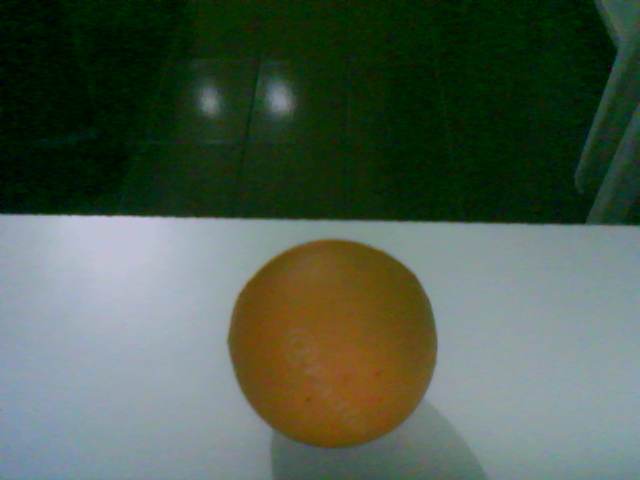
\includegraphics[scale=0.25]{figuras/cam_opencv}}
    \caption{Vídeo sendo reproduzido utilizando a biblioteca OpenCV.}
    \label{img:cam_opencv}
\end{figure}

Outra necessidade importante da aplicação desenvolvida refere-se a interação com o usuário, de modo a permitir que o mesmo seja capaz de selecionar no vídeo reproduzido pela câmera o objeto desejado para detecção e rastreamento. Para possibilitar esse recurso, desenvolveu-se uma funcionalidade onde, ao clicar com um dos botões do mouse no vídeo, a aplicação seja capaz de distinguir o objeto a ser detectado e rastreado.

A aplicação desenvolvida é composta por quatro classes, relacionadas de forma a separar a responsabilidade de cada uma delas, a fim de facilitar o entendimento do código. Esse relacionamento pode ser visto na Figura \ref{rel_sistema}.

\begin{figure}[H]
    \centering
    {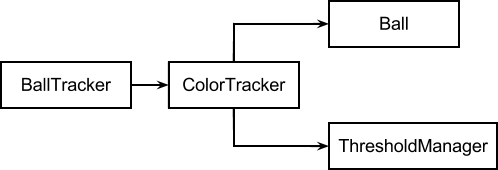
\includegraphics[scale=0.75]{figuras/rel_sistema}}
    \caption{Relacionamento entre as classes do sistema de rastreamento.}
    \label{rel_sistema}
\end{figure}

O Código \ref{code:main_sistema} mostra a inicialização do sistema. Na primeira linha de sua execução, é criado um dicionário com algumas informações pertinentes da janela, sendo elas: nome, largura e altura. Em seguida, um método do OpenCV é usado para nomear a janela a ser criada, utilizando a chave do dicionário que contém o nome desta janela. É instanciado então um vídeo, através do método do OpenCV, passando como parâmetro seu identificador.

Outras instruções no código são relacionadas a lógica para a realização do rastreamento. A criação do objeto \textit{ball\_tracker} (linha 5) tem como responsabilidade a descoberta das coordenadas do círculo, utilizando os valores do objeto a ser detectado e rastreado obtidos pelo clique do mouse. Realizada essa lógica, o objetivo final do objeto \textit{ball\_tracker} é retornar uma instância da classe \textit{Ball} (linha 10), que será utilizada pelo método \textit{circle()} do OpenCV para destacar o objeto no vídeo (linha 12 e 13). Na linha 6, é utilizado outro método da biblioteca, que gerencia os eventos do mouse na tela. Uma repetição, então, é criada com o objeto do vídeo, de forma a obter seus \textit{frames} (linha 7).

Essa implementação permite que, dentro dessa repetição, cada \textit{frame} do vídeo seja capturado e manipulado. O \textit{frame} então é recuperado (linha 8), e, caso seja válido, é usado por outros métodos. No último bloco, é feita a recuperação do objeto \textit{Ball}, contendo as coordenadas necessárias para que um círculo seja desenhado na tela. Esse objeto, então, é usado pelo método do OpenCV que circula a esfera encontrada com uma linha a sua volta e um ponto no meio, todos em azul. Por fim, o \textit{frame} desenhado é inserido na janela criada, de forma a ser visto a partir da interface com o usuário (linha 14).

\begin{code}{python}{Chamada principal do aplicativo.}{code:main_sistema}
if __name__ == '__main__':
	WINDOW_PROPERTIES = {'name': 'Visualisation', 'width': 640, 'height': 480}
	cv2.namedWindow(WINDOW_PROPERTIES['name'])
	video = cv2.VideoCapture(0)
	ball_tracker = BallTracker(video)
	cv2.setMouseCallback(WINDOW_PROPERTIES['name'], on_mouse, [ball_tracker])
	while video.grab():
		flag, frame = video.retrieve()
		if flag:
			ball = ball_tracker.get_ball(frame)
			if ball is not None:
				cv2.circle(frame, (ball.x,ball.y), ball.radius, \
					(255,0,0), 3)
				cv2.circle(frame, (ball.x,ball.y), 3, (255,0,0), -1)
			cv2.imshow(WINDOW_PROPERTIES['name'], frame)
			cv2.waitKey(1)
\end{code}

A classe \textit{BallTracker}, utilizada na chamada principal, está contida no arquivo \textit{tracker.py}, que também possui a classe \textit{ColorTracker}. A primeira, utiliza a segunda para a recuperação do objeto no vídeo baseando-se nos valores HSV do \textit{frame}.

Como ponto de partida, tem-se a chamada do método \textit{get\_ball()}, da classe \textit{BallTracker}, realizada na repetição criada pelo objeto do vídeo (Código \ref{code:get_ball}). Através desse método, é passado para a classe \textit{ColorTracker} o \textit{frame} atual do vídeo, utilizando a  função \textit{find\_ball()}. O espaço de cores desse \textit{frame} é convertido para valores HSV (Figura \ref{img:cam_hsv}) e é devidamente binarizado (Figura \ref{img:cam_bin}). Como pode ser visto no Código \ref{code:find_ball}, que contém a lógica do método \textit{find\_ball()}, são aplicados alguns filtros para melhor detecção dos contornos (linha 5). Após realizados esses tratamentos no \textit{frame}, os contornos são obtidos e utilizados para a recuperação dos parâmetros que compõem o círculo, sendo esses o centróide e raio (linha 6).\newline

\begin{code}{python}{Chamada do método da classe \textit{BallTracker} que recupera os valores do círculo baseando-se pelo \textit{frame} atual.}{code:get_ball}
def get_ball(self, frame):
	return self.color_tracker.find_ball(frame)
\end{code}

\begin{figure}[H]
	\centering
	\subfigure[\textit{Frame} do vídeo em espaço de cor HSV.]{
		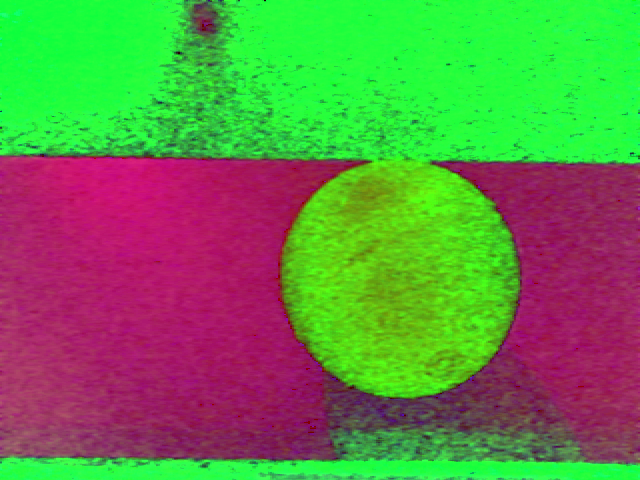
\includegraphics[scale=0.25]{figuras/cam_hsv}
		\label{img:cam_hsv}
	}\hspace{3em}
	\subfigure[\textit{Frame} após aplicação da técnica de binarização.]{
		
\includegraphics[scale=0.25]{figuras/cam_bin}
		\label{img:cam_bin}
	}
	\caption{Tratamento nos \textit{frames} do vídeo.}
	\label{img:convert_frames}
\end{figure}

\begin{code}{python}{Lógica do método \textit{find\_ball()} da classe \textit{ColorTracker}.}{code:find_ball}
def find_ball(self, frame):
	if self.manager is not None:
		hsv_frame = cv2.cvtColor(frame, cv2.COLOR_BGR2HSV)
		self.thresholded_frame = self.manager.threshold_frame(hsv_frame)
		self.thresholded_frame = self.apply_filters(self.thresholded_frame)
		return self.get_ball(self.thresholded_frame)

def get_ball(self, thresholded):
	contours, hierarchy = cv2.findContours(thresholded, cv2.RETR_TREE, \
		cv2.CHAIN_APPROX_SIMPLE)
	x, y, radius = self.get_ball_parameters(contours)
	ball = Ball(x, y, radius)
	return ball
\end{code}

Como pode ser visto no Código \ref{code:get_ball_parameters}, para a recuperação dos parâmetros do centróide e raio do círculo, é chamada a função que recupera os momentos do contorno da imagem binarizada (linha 6). Recuperado o momento do contorno, uma condição é feita para que sejam buscados os parâmetros apenas dos círculos com área maior que 1000 (linha 8). Dessa forma, evita-se que áreas do vídeo com valores HSV parecidos com o objeto desejado para detecção sejam desenhados, alcançando assim resultados mais próximos do esperado pelo usuário ao clicar com o mouse no vídeo.\newline

\begin{code}{python}{Recuperação dos valores pertinentes para identificar um círculo no \textit{frame} de vídeo.}{code:get_ball_parameters}
def get_ball_parameters(self, contours):
	(...)
	SMALLEST_OBJECT = 1000
	for contour in contours:
		try:
			moments = cv2.moments(contour)
			area = moments['m00']
			if area > SMALLEST_OBJECT:
				x = moments['m10']/area
				y = moments['m01']/area
				radius = sqrt(area/3.14)
		except:
			pass
	return x, y, radius
\end{code}

Para gerenciar o processo de binarização dos \textit{frames}, implementou-se a classe \textit{ThresholdManager}, tornando possível tratar os parâmetros do círculo e aplicá-los quando necessário. Essa classe possui em sua implementação diversas condições de mudança dos valores HSV, para que se ajustem não só a nova condição informada pelo mouse, mas também levando em conta o ambiente.

Quanto aos eventos do mouse, o OpenCV os trata através do método \textit{setMouseCallback()}, como visto anteriormente no Código \ref{code:main_sistema}, responsável por declarar um método que é chamado a cada vez que um evento do mouse é disparado. Este método deve possuir a assinatura especificada pela documentação do OpenCV, contendo o evento a ser disparado, as coordenadas x e y do mouse no vídeo, e um vetor para recuperação dos parâmetros passados pelo método \textit{setMouseCallback()}. Como pode ser visto no Código \ref{code:on_mouse},  esse valores são usados para que, ao clicar com o botão esquerdo do mouse no vídeo, os parâmetros x e y sejam passados para o método \textit{set\_hsv\_values()}. O Código \ref{code:sethsvvalues} mostra a lógica desse método, que converte o \textit{frame} do vídeo atual para o espaço de cor HSV, e através do \textit{frame} convertido, recupera o valor HSV do \textit{pixel} referente as coordenadas x e y passadas como parâmetro para o método.

\begin{code}{python}{Método que recupera informações do clique esquerdo do mouse.}{code:on_mouse}
def on_mouse(event, x, y, flag, param):
	ball_tracker = param[0]
	if event == cv2.EVENT_FLAG_LBUTTON:
		ball_tracker.set_hsv_values(x, y)
\end{code}

\begin{figure}[H]
\end{figure}

\begin{code}{python}{Converte o \textit{frame} para espaço HSV.}{code:sethsvvalues}
def set_hsv_values(self, x, y):
	flag, frame = self.video.retrieve()
	if flag:
		hsv_frame = cv2.cvtColor(frame, cv2.COLOR_BGR2HSV)
		self.color_tracker.new_value(hsv_frame[y][x][0], hsv_frame[y][x][1], \
			hsv_frame[y][x][2])
\end{code}

Dessa forma, os novos valores HSV são passados para o método \textit{new\_value()} da classe \textit{ColorTracker} (Código \ref{code:newvalue}). Em seguida, o método \textit{new\_value()} invoca a classe \textit{ThresholdManager} para que gerencie os novos valores do \textit{pixel}, e inclua-os na binarização dos próximos \textit{frames} do vídeo.

\begin{code}{python}{Um objeto do tipo \textit{ThresholdManager} é instanciado para que trate os valores HSV recuperados através do \textit{pixel} do \textit{frame}.}{code:newvalue}
def new_value(self, h, s, v):
	if self.manager is not None:
		self.manager.add_values(h, s, v)
	else:
		self.manager = ThresholdManager(h, s, v)
\end{code}

A chamada da classe \textit{ThresholdManager} é feita em dois momentos da execução do aplicativo. Na primeira vez em que a ação do clique com o mouse é realizada pelo usuário, o objeto é instanciado passando os valores HSV. Esses valores são então inicializados para criação de dois limiares, contendo valores HSV mínimos e máximos, que serão utilizados para a binarização dos \textit{frames} (Código \ref{code:init_threshold_manager}). Para os próximos eventos disparados pelo mouse, ao invés de instanciar novamente um novo objeto do tipo \textit{ThresholdManager}, o método \textit{add\_values()} é invocado pelo objeto anteriormente criado (Código \ref{code:add_values}).

\begin{code}{python}{Inicialização da classe \textit{ThresholdManager}.}{code:init_threshold_manager}
def __init__(self, h, s, v):
	self.min_h = max(0, h-1)
	self.max_h = min(179, h+1)
	self.min_s = max(0, s-1)
	self.max_s = min(255, s+1)
	self.min_v = 0
	self.max_v = 220
\end{code}

\begin{figure}[H]
\end{figure}

\begin{code}{python}{Método responsável por ajustar os valores HSV do limiares usadas para binarizar o \textit{frame} do vídeo.}{code:add_values}
def add_values(self, h, s, v):
	HUE_MARGIN = 40
	if h < (self.min_h - HUE_MARGIN):
		self.min_h -= 180
		self.max_h -= 180
	elif h > (self.max_h + HUE_MARGIN):
        h -= 180

	if h < self.min_h:
		self.min_h = h-1
	if h > self.max_h:
		self.max_h = min(179, h+1)
	if s < self.min_s:
		self.min_s = max(0, s-1)
	if s > self.max_s:
		self.max_s = min(255, s+1)
\end{code}

Através dessa estrutura lógica, ao clicar com o mouse no objeto desejado para detecção, o mesmo é contornado por um círculo azul e marcado com um ponto, indicando seu centróide. Devido as variações das cores do objeto a ser detectado, causadas pela luminosidade do local, procura-se escolher áreas do objeto contendo cores mais homogêneas. Dessa forma, resultados mais precisos são alcançados, como visto na Figura \ref{img:cam_final}.

\begin{figure}[H]
    \centering
    {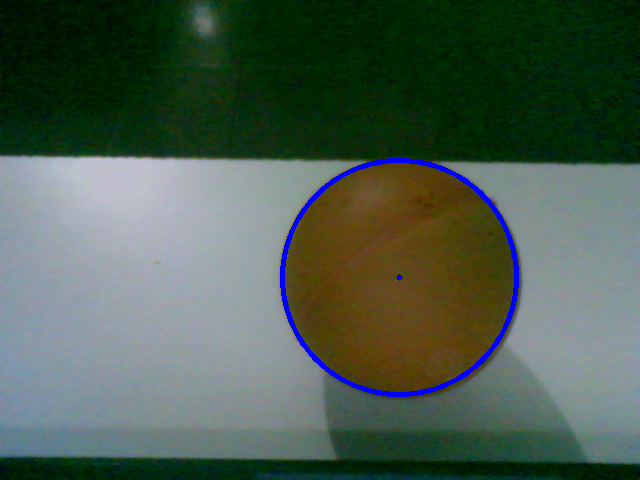
\includegraphics[scale=0.25]{figuras/cam_final}}
    \caption{Resultado final do sistema, detectando uma bola laranja na tela e circulando-a.}
    \label{img:cam_final}
\end{figure}

\section{Resultados}

Como modelo de objeto para detecção e rastreamento, utilizou-se uma bola laranja. Esse objeto foi utilizado em dois planos de fundo, um monocromático e outro policromático. Nesses dois casos, situações foram testadas com o objeto parado e em movimento na cena.

Em um plano de fundo básico, os ajustes dos limiares puderam ser feitos baseando-se em diferentes contrastes de cores referentes ao objeto. Dessa forma, a detecção se mostrou precisa, como mostra a Figura \ref{img:res_basico_parado}, estando o objeto completamente parado. Expondo o mesmo objeto em diferentes velocidades de movimentação no vídeo, os resultados mostraram-se satisfátorios (Figura \ref{img:res_basico_mov}). Em casos onde o objeto se desloca lentamente, o círculo que denota a detecção não possuiu a mesma precisão, porém apresentou um raio de dimensão próxima a original (Figura \ref{img:res_basico_mov1}) (Figura \ref{img:res_basico_mov2}). Nos casos onde o objeto se desloca mais rapidamente, a tendência é que a detecção seja feita acompanhando a tragetória do objeto, porém com precisão menor, fazendo com que o círculo representativo da detecção diminua (Figura \ref{img:res_basico_mov3}).

\begin{figure}[H]
    \centering
    {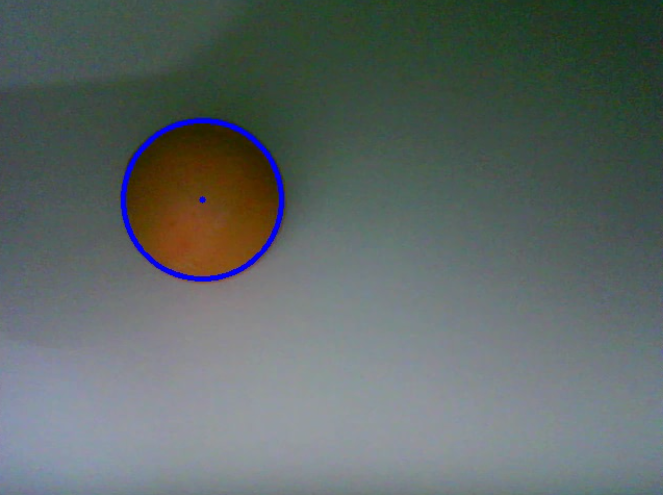
\includegraphics[scale=0.25]{figuras/res_basico1}}
    \caption{Caso básico de detecção, com o objeto parado no vídeo.}
    \label{img:res_basico_parado}
\end{figure}

\begin{figure}[H]
	\centering
	\subfigure[Detecção com pouco deslocamento do objeto.]{
		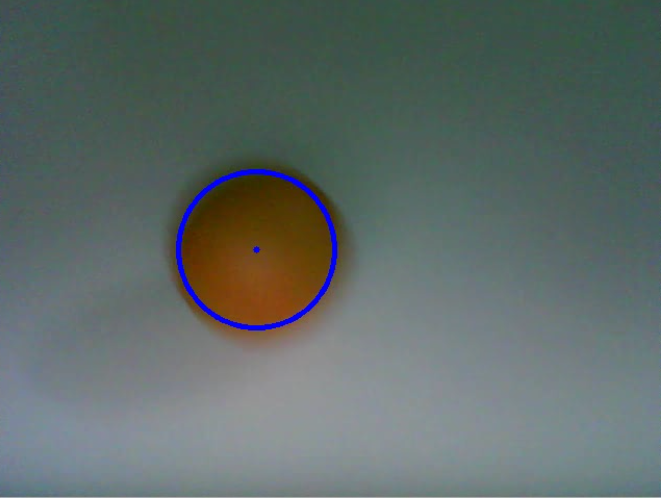
\includegraphics[scale=0.25]{figuras/res_basico_mov1}
		\label{img:res_basico_mov1}
	}\hspace{3em}
	\subfigure[Detecção com médio deslocamento do objeto.]{
		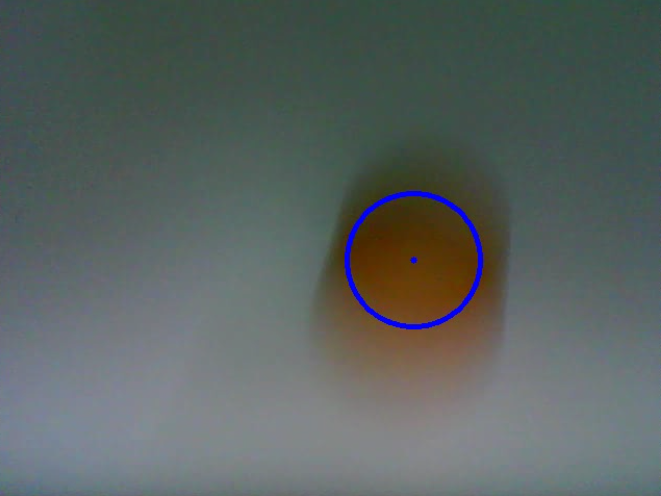
\includegraphics[scale=0.25]{figuras/res_basico_mov2}
		\label{img:res_basico_mov2}
	}\hspace{3em}
	\subfigure[Detecção com muito deslocamento do objeto.]{
		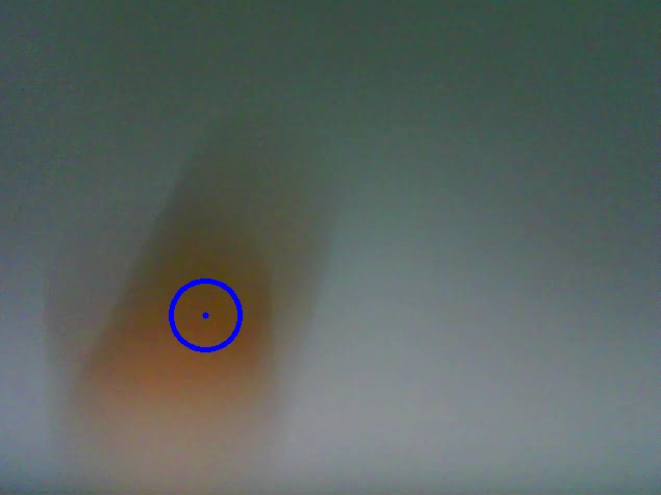
\includegraphics[scale=0.25]{figuras/res_basico_mov3}
		\label{img:res_basico_mov3}
	}
	\caption{Diversos testes feitos com o objeto em diferentes velocidades.}
	\label{img:res_basico_mov}
\end{figure}

Nos casos em que foi utilizado um plano de fundo policromático, a detecção se manteve precisa. Ajustando os limiares com base no novo plano de fundo, o objeto foi rastreado, porém com intermitências em sua detecção. A Figura \ref{img:res_complexo} apresenta casos em que o objeto foi exposto em diferentes distâncias em relação ao vídeo, estando em movimento. Apesar do objeto se apresentar em contraste parecido com o fundo, a aplicação mostrou qualidade na precisão, separando o objeto do plano de fundo complexo.

\begin{figure}[H]
	\centering
	\subfigure[Detecção com o objeto parado em um plano de fundo complexo.]{
		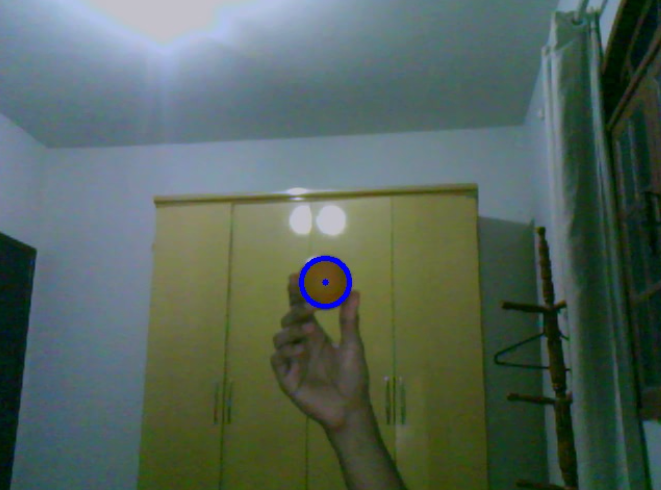
\includegraphics[scale=0.25]{figuras/res_complexo1}
		\label{img:res_complexo1}
	}\hspace{3em}
	\subfigure[Detecção com o objeto em movimento próximo ao vídeo.]{
		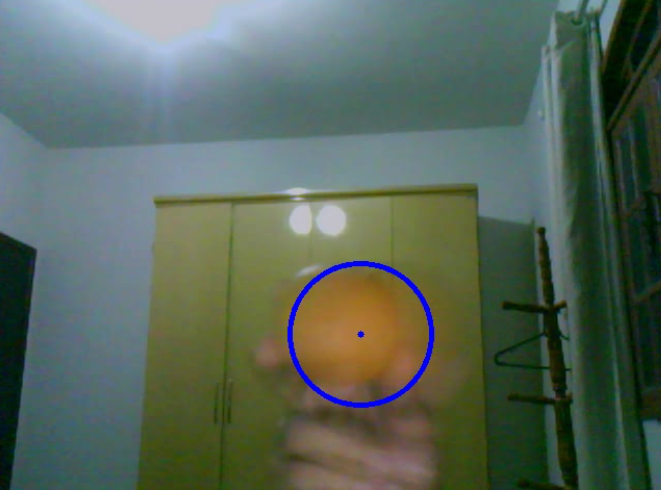
\includegraphics[scale=0.25]{figuras/res_complexo_mov1}
		\label{img:res_complexo_mov1}
	}\hspace{3em}
	\subfigure[Detecção com o objeto em movimento afastado do vídeo.]{
		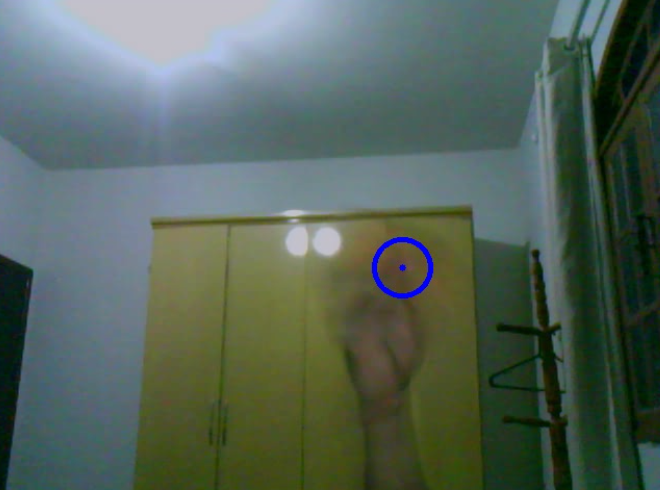
\includegraphics[scale=0.25]{figuras/res_complexo_mov2}
		\label{img:res_complexo_mov2}
	}\hspace{3em}
	\subfigure[Detecção com o objeto em distância média do vídeo.]{
		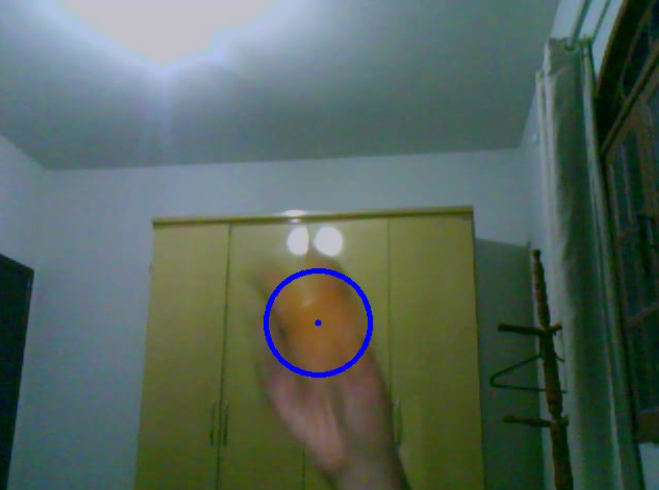
\includegraphics[scale=0.25]{figuras/res_complexo_mov3}
		\label{img:res_complexo_mov3}
	}
	\caption{Diversos testes feitos com o objeto em um plano de fundo complexo, em diferentes proximidades com o vídeo.}
	\label{img:res_complexo}
\end{figure}

No entanto, em alguns casos com o objeto sendo deslocado rapidamente, a detecção não foi feita, assim como nos casos testados com plano de fundo básico (Figura \ref{img:res_complexo_fail}). Apesar de não terem sido realizados testes mais aprofundados, a utilização de equipamentos mais sofisticados para a captura do vídeo e processamento da aplicação podem ocasionar em resultados mais satisfatórios na detecção do objeto.

\begin{figure}[H]
    \centering
    {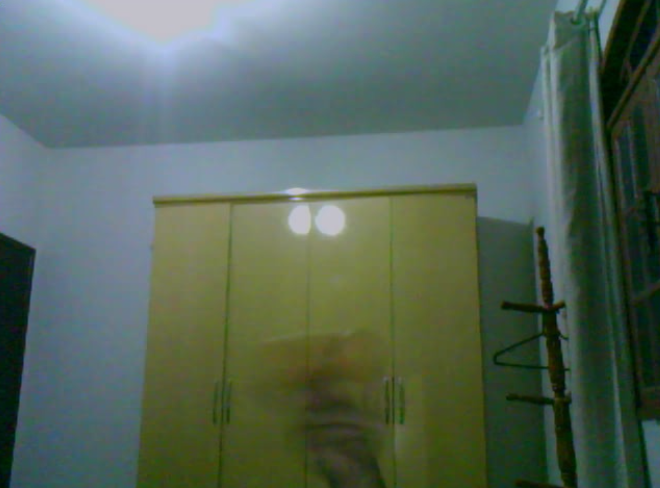
\includegraphics[scale=0.25]{figuras/res_complexo_fail}}
    \caption{Em alguns momentos, a aplicação falhou em detectar o objeto desejado.}
    \label{img:res_complexo_fail}
\end{figure}

Outros casos ainda foram testados considerando outros fatores como iluminação e o objeto não sendo mostrado por completo no vídeo. Os casos em que o objeto é colocado próximo a luz, a aplicação passou a não detectá-lo (Figura \ref{img:res_complexo_luz}). Por terem sido utilizados limiares com base nos tons laranja do objeto, ao aproximá-lo da luz, o tom de cor do mesmo é alterado. Nesses casos, para a correta detecção, é necessário reajustar os limiares de modo a considerar esses novos tons de cores do objeto próximos a luz. Contudo, ao realizar esses ajustes, corre-se o risco da aplicação considerar outros objetos na cena, por possuírem o mesmo tom de cor do objeto.

\begin{figure}[H]
    \centering
    {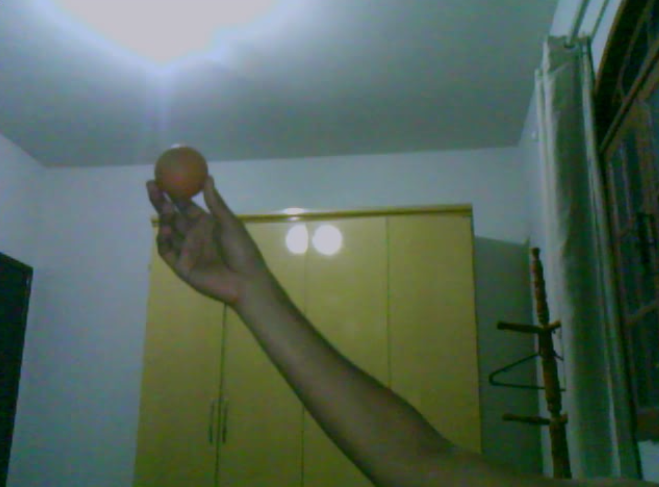
\includegraphics[scale=0.25]{figuras/res_complexo_luz}}
    \caption{Aproximando o objeto da luz artificial, a tendência é que a detecção também falhe.}
    \label{img:res_complexo_luz}
\end{figure}

Nas situações onde o objeto foi apresentado parcialmente no vídeo, os resultados foram positivos. A Figura \ref{img:res_complexo_obst} apresenta alguns casos onde o objeto foi apresentado com alguns obstáculos.

\begin{figure}[H]
	\centering
	\subfigure[Caso em que detecção foi bem sucedida mesmo sendo mostrada parcialmente no vídeo.]{
		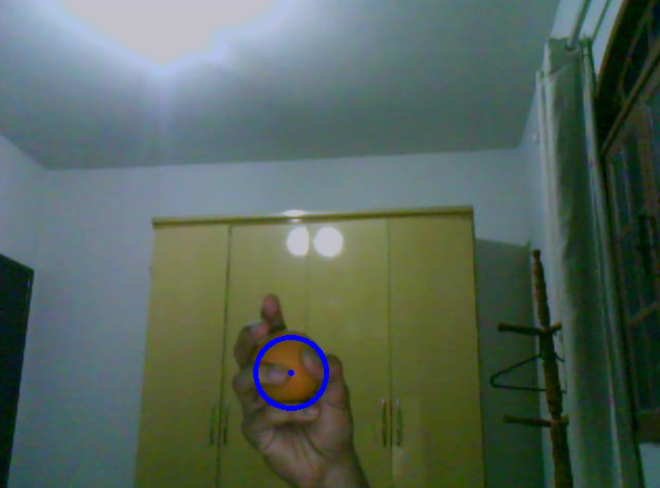
\includegraphics[scale=0.25]{figuras/res_complexo_obst1}
		\label{img:res_complexo_obst1}
	}\hspace{3em}
	\subfigure[Segundo caso onde o resultado foi positivo para detecção com obstáculos.]{
		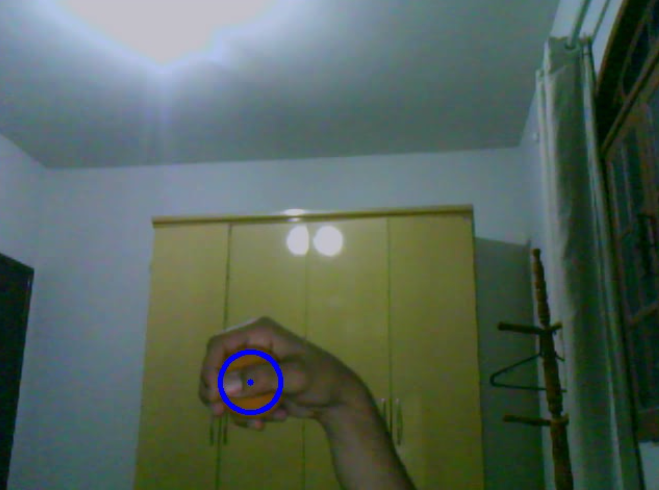
\includegraphics[scale=0.25]{figuras/res_complexo_obst2}
		\label{img:res_complexo_obst2}
	}
	\caption{Casos de sucesso na detecção do objeto em situações adversas.}
	\label{img:res_complexo_obst}
\end{figure}
 % ESTUDO DE CASO
	\chapter{CONCLUSÕES}

Este trabalho possibilitou a criação de uma documentação sucinta da área de Visão Computacional, reunindo as principais técnicas utilizadas para o desenvolvimento de aplicações na área. As pesquisas relacionadas ao desenvolvimento desses sistemas tiveram como objetivo agregar as principais ferramentas de linguagem Python utilizadas atualmente. Como resultado dessas pesquisas, descobriu-se que o OpenCV é uma ótima opção para o desenvolvimento de aplicações na área de Visão Computacional em linguagem Python, contendo diversos materiais e livros descrevendo suas funcionalidades. Do mesmo modo, as pesquisas voltadas para o \textit{framework} SimpleCV mostraram a ferramenta como um complemento que simplifica o desenvolvimento de sistemas de Visão Computacional.

Com a utilização de exemplos práticos utilizando essas ferramentas, foi possível apresentar conceitos da área de Visão Computacional normalmente vistos de forma abstrata nos principais materiais desse domínio de estudo. Com isso, o trabalho também permitiu a aproximação entre o domínio da Visão Computacional e profissionais da computação, compondo uma base de consulta para o estudo e desenvolvimento de trabalhos futuros.

Através das pesquisas para o desenvolvimento da aplicação mostrada como estudo de caso, percebeu-se que as ferramentas da área de Visão Computacional para Python estão maduras o bastante para que pessoas com interesse, na área da computação, possam utilizá-las para o desenvolvimento de aplicações.

O estudo de caso obteve sucesso na criação de uma aplicação para detecção e rastreamento de objetos circulares monocromáticos, possibilitando a recuperação de informações pertinentes do mesmo. Dessa forma, possíveis funcionalidades podem ser criadas, como por exemplo estimar o quão distante o objeto está em relação ao vídeo, baseando-se no raio do objeto circular, obtido através dos cálculos feitos pela aplicação.

A base do que foi desenvolvido para a criação do estudo de caso pode ser aplicada em projetos de maior complexidade que visam resolver problemas cotidianos. Exemplos de projetos que podem utilizar a mesma base do que foi desenvolvido são aplicados em áreas de segurança e esportes. Através da detecção de bolas em esportes como futebol e tênis por exemplo, é possível determinar quanto tempo a bola esteve em jogo, ou então concluir se a bola tocou o lado de dentro ou fora da quadra. Em áreas da segurança, mais especificamente a área de autenticação, a utilização da lógica de detecção de objetos circulares pode ser aplicada para reconhecimento do globo ocular, visando avaliá-lo biometricamente para credenciar a entrada de pessoas em áreas restritas.

Este projeto permite também que outros trabalhos futuros possam ser elaborados, como por exemplo, utilizar o Arduino\footnote{Plataforma de hardware e software livre que simplifica a criação e prototipagem de projetos de eletrônica.} visando integrar a aplicação com robôs para que possam se guiar a partir do objeto detectado pela aplicação. Ainda, estimando a distância do objeto em relação ao vídeo, pode-se criar uma inteligência capaz de permitir que o robô ande mais rápido se o objeto estiver distante do vídeo, e de mesma forma, ande mais devagar se o objeto estiver próximo.

Conclui-se, então, que o desenvolvimento de aplicações da Visão Computacional pode ser otimizado com a utilização de tecnologias atuais, possibilitando a criação de aplicações na área de Visão Computacional com maior rapidez. Dessa forma, projetos são mais facilmente desenvolvidos, popularizando ainda mais a área de Visão Computacional.
 % CONCLUSÕES
	\bibliographystyle{abnt-alf}
	\bibliography{referencia} % Gera as referências bibliográficas
\end{document}
